\documentclass[a4paper,9pt]{article}
%\documentclass{aa}
%\pgfplotsset{compat=1.12}
\usepackage{conference}
\usepackage{latexsym}
\usepackage[perpage,symbol*]{footmisc}
%\usepackage[utf8]{inputenc}
\usepackage[utf8x]{inputenc}
\usepackage{textcomp}
\usepackage[english]{babel}
\usepackage{amssymb,amsfonts,amsmath}
\usepackage{xcolor}

%\usepackage{graphicx}
%\usepackage{pstricks,pst-node}             % Pstricks
\usepackage{tikz}
\usepackage{tikz-3dplot}
\usepackage{pgfplots}
\usepackage{pgfplotstable}

\usepackage{cite}
\usepackage{hyperref}
\usepackage[varg]{txfonts}
\usepackage{booktabs}       % professional-quality tables
%\usepackage[letterpaper, landscape, lmargin=0.25in, rmargin=1.25in]{geometry}
\usepackage{tabularx}
\usepackage{enumerate}
%\usepackage{enumitem}
\usepackage{multicol}
% \usepackage{ifpdf}

% \usetikzlibrary{shapes}
% \usepackage[left=0.1cm, right=0.1cm, top=0.1cm, bottom=0.1cm]{geometry}
% \usepackage[ansinew]{inputenc}           % Input
\usepackage[T1]{fontenc}                   % Font encoding
% \usepackage{cmbright}                    % Font style
%\usepackage[nohead,margin=0mm]{geometry}  % Page & margins

%%%%%%
%%%%%%

\usetikzlibrary{patterns,arrows.meta,calc,angles,positioning,intersections,through,quotes,decorations.markings}
\usepackage{tkz-euclide}
\usetkzobj{all}

\newcommand\RectTri[4][thick,green!50!black,text=black]{%
\coordinate [label=left:$C$] (C) at #2;
\coordinate [label=below right:$B$] (B) at #3;
\coordinate (aux) at ($ #2 ! 1 ! 90:#3 $);
\coordinate [label=above:$A$] (A) at ($ #2 !#4!(aux) $);

\coordinate (perp) at ($(A)!(C)!(B)$);
\draw[purple!70!black,thick,dashed] (C) -- (perp);

\draw[#1] 
  (C) -- 
  node[auto] {$\sqrt{a''}$} (A) -- 
  node[auto] {$\sqrt{a}$} (B) --
  node[auto] {$\sqrt{a'}$} 
  (C)
  pic ["$\theta$",draw,red,thick,angle radius=1cm] {angle = C--A--B} 
  pic ["$\alpha$",draw,cyan,thick,angle radius=1cm] {angle = B--C--perp}
  pic ["$\beta$",draw,orange!70!black,thick,angle radius=1cm] {angle = A--B--C}
  pic ["$\beta$",draw,orange!70!black,thick,angle radius=1cm] {angle = perp--C--A};
}

\tikzset{
mydot/.style={
  fill,
  circle,
  inner sep=1.5pt
  }
}

%%%%%%%
%%%%%%%
%%%%%%%

%% Begin of Watermark feature
%\usepackage[printwatermark]{xwatermark}
%\usepackage{xcolor}
%\newwatermark[allpages,color=red!50,angle=60,scale=6,xpos=0,ypos=0]{DRAFT}
%\newwatermark[allpages,color=red!20,angle=60,scale=2,xpos=0,ypos=0]{For Peer Review}
%% End of Watermark feature

%\pagenumbering{gobble}

\title{Towards Physics-Arithmetics Unification}

\author{F. M. Sanchez \thanks{Retired Prof. of Physics, University of Paris 11, Orsay, France, \href{mailto:hol137@yahoo.fr}{hol137@yahoo.fr}} 
   %%\\ email \href{mailto:hol137@yahoo.fr}{hol137@yahoo.fr}  	  
   \and M. H. Grosmann \thanks{Retired Prof. of Physics, University of Strasbourg, France, \href{mailto:michelgrosmann@me.com}{michelgrosmann@me.com}}
   %%\\ email \href{mailto:michelgrosmann@me.com}{michelgrosmann@me.com} 
   \and R. Veysseyre \thanks{Retired Agregee de mathematiques et professeur honoraire \`a l'Ecole centrale de Paris, France, \href{mailto:renee.veysseyre@normalsup.org}{renee.veysseyre@normalsup.org}}
   %%\\ email \href{mailto:renee.veysseyre@normalsup.org}{renee.veysseyre@normalsup.org} 
   \and D. Weigel  \thanks{Retired Prof of Cristallography, University of Paris 6, Paris, France, \href{mailto:dominiqueweigel18@gmail.com}{dominiqueweigel18@gmail.com}} 
   %%\\ email \href{mailto:dominiqueweigel18@gmail.com}{dominiqueweigel18@gmail.com} 
   \and L. Gueroult \thanks{Retired PhD instructor in Holography at ENS, Physics department A2, Cachan, France, \href{mailto:lgueroult@hotmail.com}{lgueroult@hotmail.com}}
   %%\\ email \href{mailto:lgueroult@hotmail.com}{lgueroult@hotmail.com}
   }

\begin{document}
\setcounter{page}{1}

\maketitle

\begin{abstract}
The hypothesis that the Cosmos is a computer leads to a reunification of Arithmetics and Physics, through a systematic optimisation and symbolic rationalisation process, the later being a kind of renormalisation, in the sense that this minimizes the number of parameters. The $\pi$ symbolic rationalisation rehabilitates the Wyler's theory and confirms in the ppb domain the G value deduced from Permanent Cosmology, excluding the concept of universe expansion. With the hypothesis that the scalar massive boson is $495^2$ times the electron mass, the tau value from Koide Fermion formula connects with the electroweak model. 

\end{abstract}


% keywords can be removed
\keywords{Quantum Physics \and Quantum Gravity \and String Theory \and Number theory \and Cosmology \and Holography \and Holic Principle \and Crystallography}



\label{sec:headings}

\tableofcontents




\section{L’inversion des constantes de couplages}
Dans la théorie standard, on procède par approximations successives, c’est la méthode dite ’’des perturbations’’. Ainsi le "couplage électrique" standard est un  nombre inférieur à l’unité, de sorte qu’on puisse négliger son influence à des puissances suffisantes. On a pris l’habitude de le désigner par la lettre $\alpha$, appelée ‘constante de structure fine’, car ce nombre aparaît dans l’étude des raies spectrales, jusqu’à des puissances cinquièmes et plus. Il est lié à la charge électrique, mais la notation courante de celle-ci $e$ peut entrainer des confusions avec la base optimale des logarithmes néperiens, qui est d’importance centrale dans le cadre d’un cosmos calculateur, qui est l'hypothèse centrale de cet article où la charge électrique élémentaire est donc notée $q$. Un tel Cosmos calculateur doit utiliser des bases de calcul supérieures à l’unité, donc les 4 constantes de couplages (électrique, gravitationnelle, faible, forte) notées $a, a_G, a_w, a_s$, sont les inverses des quantités officielles (table 1). Les constantes physiques sont rassemblées dans la table 2 \cite{Tanabashi}. 



\section{L'exigence de quasi-continuité : la rationalisation symbolique de $\pi$} 
La physique mathématique fait face à une crise grave. Le modèle standard des particules est incapable d’inclure la gravitation, se heurtant à des problèmes de renormalisation, c’est-à-dire l’élimination de quantités infinies qui apparaissent dans les calculs. Nous proposons ici l’hypothèse d’une rationalisation symbolique de $\pi$, revenant à supprimer les décimales infinies de $\pi$ au-dela d’un certain nombre. 

Cette hypothèse a été présentée comme une "exigencede quasi-continuité" dans une conférence à Cambridge en 1994 \cite{Sanchez1}, introduisant le Principe Holographique. En effet, par opposition aux équations différentielles, les équations globales les plus simples sont les connexions entre variétés topologiques de dimensions différentes (périmètre, aire, volume…), donc utilisent la constante $\pi$.  

Dans l’hypothèse d’un Cosmos calculateur, de même qu’un ordinateur ne peut utiliser le $\pi$ mathématique "rigoureux", tout calcul doit être associé à une imprécision. Dans cet article, la précision maximale $10^{-9}$ (ou ppb) est recherchée, laissant peu de prise au hasard. Ainsi $\pi$ \textit {doit} être rationalisé, et, dans un premier temps, de manière symbolique, c’est-à-dire que son développement fractionnaire doit montrer des paramètres-clefs.

En effet, le développement fractionaire dU $\pi$ mathématique commence par les nombres 3, 7, 15, 1, 292.634, ce dernier terme étant le rapport de masse neutron/électron divisé par $2\pi$, à 3 ppm près. Le développement partiel suivant:

\begin{equation}
\pi_n : 3, 7, 15, 1, n/2\pi  
 \end{equation}

définit le $\pi$ mathématique à mieux que le ppb. La suite fractionnaire de $\pi$ est un problème non résolu des mathématiques actuelles. Cependant on note que le nombre $292$ est la moyenne des nombres de symétries paires (419) et impaires (265) dans l'espace des supercordes $10D$ \cite{Weigel} \cite{Veysseyre}(table 1).


Avec la valeur de $G$ optimisée par une étude de corrélation \cite{Sanchez2} (table 2), on observe la relation suivante entre les trois paramètres de couplages électrique, électrofaible et gravitationnel $a, a_w, P$ (table 3):

\begin{equation}
a_w^{5/2} \approx (419/417) P a^3  
 \end{equation}

précise au ppb, où $417 = 419 - 2$ est le nombre de symétries positives $10D$ non triviales.

De plus, la masse gravitationnelle du proton $p_G = P/\sqrt {N_L}\approx 1831.531182$, où $N_L$ est le grand nombre de Lucas, le terme terminal de a Hiérarchie Combinatoire \cite{Bastin}, écrite sous la forme de Lenz-Wyler \cite{Wyler}, présente un développement singulier: 

\begin{equation}
p_G = 6\pi_G^5~~~~ \rightarrow  ~~~~ \pi_G : 3, 7, 7, 7\sqrt 7
\end{equation}

Cette formule, précise à 5 ppb, est caractéristique de l'algèbre des octonions. \textit{Sir Atiyah avait effectivement annoncé que la gravitation devait être liée à cet algèbre}\cite {Atiyah}:
 
A noter que ce nombre $p_G$ se trouve aussi dans le développement suivant de $e : 2, 7/5, -3\sqrt{p_G}$. Ce développement est basé sur l'approximation $e \approx 19/7$, qui connecte avec l'approximation d'Archimède: $\pi \approx 22/7$
 
\begin{table}
\label{tab:10:table10}
%% \caption{Table 3: }
  \hskip-0.0cm\begin{tabular}{llllllllllllll}
    \toprule
    \multicolumn{14}{c}{Table 3. Crystallographic $PSO_{Cr}$}                  \\
    \cmidrule(r){1-14}
    %\ $E^d$ & E & $E^1$  & $E^2$ & $E^3$ & $E^4$ & $E^5$ & $E^6$ & $E^7$ & $E^8$ & $E^9$ & $E^{10}$ & $E^{11}$ & $E^{12}$ \\
    \midrule
    %$K_{d+}$  & 1 & 1 & 5 & 5 & 19 & 19 & 59 & 59 & 165 & 165 & 419 & 419 & 1001 \\
    
     %$K_{d-}$  &  & 1 & 1 & 5 & 5 & 19 & 19 & 59 & 59 & 165 & 165& 419 & 419 \\
     
    % $2K_{d+} + K_{d-}$  & 2 & 3 & 11 & 15 & 43 & 57 & 137 & 177 & 389 & 495 & 1003 & 1257& 2421 \\
     
      %$(K_{d+} - K_{d-})/2 + d$  &  &  & 4 & 3 & 11 & 5 & 26 & 7 & 61 & 9 & 137 & 11& 303 \\
      
      \ $E^{(d)}$ & $E^{(0)}$ & $E^{(1)} $ & $E^{(2)}$ & $E^{(3)} $& $E^{(4)}$ &$ E^{(5)}$ &$ E^{(6)} $&$ E^{(7)}$ &$ E^{(8)}$ & $E^{(9)}$ &$ E^{(10)} $&$ E^{(11)} $&$ E^{(12)}$ \\
    \midrule
    $K_{d+}$  & 1 & 1 & 5 & 5 & 19 & 19 & 59 & 59 & 165 & 165 & 419 & 419 & 1001 \\
    
     $K_{d-}$  &  & 1 & 1 & 5 & 5 & 19 & 19 & 59 & 59 & 165 & 165& 419 & 419 \\
     
      $K_{d} = (K_{d+} + K_{d-})/2$  & & 1 & 3 & 5 & 12 & 19 & 39 & 59 & 112 & 165 & 292 & 419 & 710 \\
      
      $\Sigma K_{d}$ &  & 1 & 4 & 9 & 21 & 40 & 79 & 138 & 250 & 415 & 707 & 1126 & 1836 \\
      
      $K_{(d-1)+} +K_{d+}+ K_{(d+1)+}$  &  & 7 & 11 & 29 & 43 & 97 & 137 & 283 & 389 & 749 & 1003 & 1839 & 2421 \\

    \bottomrule
  \end{tabular}
\end{table}



\section{La théorie bosonique des cordes et le rayon \textit{invariant} de Hubble}
La théorie des cordes a suscité un espoir énorme quand elle a exhibé une particule de spin 2, qu'on a identifié au graviton, intégrant ainsi la gravitaton. De plus, elle a mis en évidence une correspondance holographique explicite entre des espaces-temps $5D$ et $4D$.  \textit{Mais cete théorie bute sur le concept de l'univers en expansion}. 

La plupart des physiciens ont opté pour la soluton de facilité, le "Multivers", évacuant le problème épineux de la caractérisation précise de l'Univers. Ils s'appuient sur le fait que le nombre de solutions pour le repliement des dimensions cachées  est énorme ($10^{500}$). 


Mais cela est firtement discuté actuellement, et remis en question par une étude précédente \cite{Sanchez2} qui a montré que les multiples corrélations observées entre les grands nombres de la physique mathématique pouvait être considérées comme une succession de relations holographiques 1D-2D, aboutissant à l'Axe Topologique (Fig 1), confirmant la théorie bosonique des cordes, et sa dimension 26, qui correspond au rayon de Hubble donné par le modèle de la molécule gravitationnelle d'hydrogène $R =  2 \hbar^2/Gm_e m_p m_H \approx 13.812 \times 10^3$ années-lumère, compatible avec les mesures directes du rayon de Hubble qui contredisent la cosmologie standard de 10% \cite{Tanabashi}.


En effet, cette valeur de $R$ connecte avec la fonction topologique réduite : $g(k) = exp(2^{k+1/2})/k$, pour la valeur $k = 6 (d = 26)$ de l'Axe Topologique, où $26$ est la dimension privilégiée de la thèorie bosonique des cordes: 

\begin{equation}
R/\lambdabar_e \approx g(6)
 \end{equation}

où $\lambdabar_e = \hbar/m_ec$ est la longueur d'onde réduite de l'électron. Les multiples relations holographiques, impliquant en particulier le rayonnement de fond, qui est donc aussi invariant, conduisent à:

\begin{equation}
R/\lambdabar_e \approx (2\pi^2a^3)^5
 \end{equation}

où $2\pi^2a^3$ est l’aire de la sphère 4D de rayon $a$, mais cette relation montre une imprécision de 565 ppm. On constate que la déviaton ci-dessus est voisine de $H/p_W$, à 1.5 ppm près. Et ce dernier écart est réduit au ppb si on considère la valeur suivante de $\pi$:

\begin{equation}
\pi_R = 3 + 1/(7+1/(16+2/e^{2e})
\end{equation}

Noter que $H ≈ 8e^{2e}$ à 33 ppm près. On retrouve ainsi, à $10^{-9}$ près, la valeur $R ≈ 13.8119768$ milliards d’années-lumière :

\begin{equation}
R/\lambdabar_e  \approx H (2\pi_R a^3)^5
\end{equation}

ce qui rétablit une symmétrie électron-hydrogène, conformément au modèle de la molécule gravitationnelle d’hydrogène. 


La table 4 présente 14 formules au ppb pour ce rayon de Hubble. Cette démarche rappelle celle de Jean Perrin qui en présentant 14 formules impliquant des nombes de molécules a convaincu la communauté de l'existence réelle ds atomes.






\begin{figure}
%\label{fig:figure_label}
\label{tab:9:table9}
\centering
\includegraphics[width=\textwidth,height=14cm]{./figure/figure}
\caption[The Topological Axis]
{This is the extrapolation toward smaller numbers of the Eddington's Double Larger Number correlation. The double natural logarithms y = ln(ln(Y)) of the main dimensionless physical quantities (Y) corresponds to the special string dimension series d = 4k + 2, from k = 0 to k = 7, characteristics of a Bott octonion sequence. This is the reunion of height 2D-1D holographic relations, hence the name `Topological Axis`.}
%%Two relations come from the double large number correlation \cite{Eddington}, the first one comes from the Carr and Rees weak boson-gravitation relation\cite{Carr}, while the other comes from the Davies analysis, which involvies the Cosmological Microwave Background (CMB) wavelength. \textit{In the macro-physics side, with length unit  the Electron Compton reduced wavelength $\lambdabar_e$}, $6 \times$ the Hubble radius 13.812 billion light-years, is tied to the bosonic critical dimension 26 (k = 6), while Bott reduction $\Delta$d = 8 leads firstly to  d = 18: it is the \textit{thermal photon} (CMB). This temperature $T \approx 2.7258 Kelvin$, is identified to the common temperature of the couple Universe-Cosmos. It is tied to the the mammal wavelength through the Sternheimer scale factor $j$ \cite{Sternheimer}; another Bott reduction leads to d = 10 (super-string dimension): it is the \textit{Hydrogen atom}, and finally to d = 2: the \textit{massive string}, about 2.1 GeV. For the number 24 of transverse dimensions, it is the \textit{non-Doppler sun-quasar Kotov length}, multiplied by a factor about 2$\pi a$, with $a \approx 137.036$. For d $\approx \Gamma$, the Atiyah constant \cite{Atiyah}, it is the \textit{galaxy group} radius, a characteristic cosmic length ($10^{6}$ light-years. For k $\approx e^{2}$, $y \approx 2e$, it is the \textit{Cosmos} radius. The Space-Time-Matter Holic dimension d = 30 is tied to $c$ times the cosmic \textit{Supercycle period}. \textit{In the micro-physics side, with the same length unit $\lambdabar_e$}, Bott octonion reductions from d = 30 lead  to the \textit{gauge bosons}. Firstly d = 22 corresponds to the Grand Unification Theory (GUT) one, ($ 2.30\cdot10^{16}$ GeV). Secondly d = 14 corresponds to the weak ones. Finaly d = 6 corresponds to (\textit{massive}) gluons, about 8.6 MeV. For the intermediary superstring value d = 10, there is the mean \textit{Pion}. For d $\approx \gamma \times \Gamma$, Y $\approx 495^2$ the square of the diminished Green-Schwarz string dimension (496 - 1), it is the \textit{Brout-Englert-Higgs boson} (125.175 GeV). For k $\approx 2e^e$, it is the \textit{topon}, the visible Universe wavelength, the space quantum, which identifies with the mono-radial unit length of the Bekenstein-Hawking Universe entropy (section 3). \textit{With unit $2\pi$ times the Nambu mass $m_N~=~am_e$}, d = 24 and 26 corresponds to the \textit{photon and graviton masses}, defined by the two-step holographic interaction\cite{Sanchez1}.} The central dimension is d = 16, for a total of $2^7$ string dimensions in the Bott sequence. It suggests a liaison with the Eddigton's matrix $16 \times 16$ \cite{Eddington}.}
%% {This is the extrapolation towards smaller numbers of the Eddington's Double Larger Number correlation. The double natural logarithms y = ln(ln(Y)) of the main dimensionless physical quantities (Y) corresponds to the special string dimension series d = 4k + 2, from k = 0 to k = 7, characteristics of a Bott octonion sequence. This is the reunion of height 2D-1D holographic relations, hence the name `Topological Axis`. Two relations come from the double large number correlation \cite{Eddington}, the first one comes from the Carr and Rees weak boson-gravitation relation\cite{Carr}, while the other comes from the Davies analysis, which involvies the Cosmological Microwave Background (CMB) wavelength. \textit{In the macro-physics side, with length unit  the Electron Compton reduced wavelength $\lambdabar_e$}, $6 \times$ the Hubble radius 13.812 billion light-years, is tied to the bosonic critical dimension 26 (k = 6), while Bott reduction $\Delta$d = 8 leads firstly to  d = 18: it is the \textit{thermal photon} (CMB). This temperature $T \approx 2.7258 Kelvin$, is identified to the common temperature of the couple Universe-Cosmos. It is tied to the the mammal wavelength through the Sternheimer scale factor $j$ \cite{Sternheimer}; another Bott reduction leads to d = 10 (super-string dimension): it is the \textit{Hydrogen atom}, and finally to d = 2: the \textit{massive string}, about 2.1 GeV. For the number 24 of transverse dimensions, it is the \textit{non-Doppler sun-quasar Kotov length}, multiplied by a factor about 2$\pi a$, with $a \approx 137.036$. For d $\approx \Gamma$, the Atiyah constant \cite{Atiyah}, it is the \textit{galaxy group} radius, a characteristic cosmic length ($10^{6}$ light-years. For k $\approx e^{2}$, $y \approx 2e$, it is the \textit{Cosmos} radius. The Space-Time-Matter Holic dimension d = 30 is tied to $c$ times the cosmic \textit{Supercycle period}. \textit{In the micro-physics side, with the same length unit $\lambdabar_e$}, Bott octonion reductions from d = 30 lead  to the \textit{gauge bosons}. Firstly d = 22 corresponds to the Grand Unification Theory (GUT) one, ($ 2.30\cdot10^{16}$ GeV). Secondly d = 14 corresponds to the weak ones. Finaly d = 6 corresponds to (\textit{massive}) gluons, about 8.6 MeV. For the intermediary superstring value d = 10, there is the mean \textit{Pion}. For d $\approx \gamma \times \Gamma$, Y $\approx 495^2$ the square of the diminished Green-Schwarz string dimension (496 - 1), it is the \textit{Brout-Englert-Higgs boson} (125.175 GeV). For k $\approx 2e^e$, it is the \textit{topon}, the visible Universe wavelength, the space quantum, which identifies with the mono-radial unit length of the Bekenstein-Hawking Universe entropy (section 3). \textit{With unit $2\pi$ times the Nambu mass $m_N~=~am_e$}, d = 24 and 26 corresponds to the \textit{photon and graviton masses}, defined by the two-step holographic interaction\cite{Sanchez1}.} The central dimension is d = 16, for a total of $2^7$ string dimensions in the Bott sequence. It suggests a liaison with the Eddigton's matrix $16 \times 16$ \cite{Eddington}.}
\end{figure}

\begin{figure}
\centering
\includegraphics[width=5cm,height=6cm]{./figure/triaxis.png}
\caption[MLT Geodimensional cuboid]{\textit{Geo-dimensional Universe-Grandcosmos couple}, with unit length the Electron Compton reduced wavelength. 
In a 3D Super-space, logarithms of physical ratios are considered vectors. The Grandcosmos radius appears as the norm of the vector using for length and time projections the same value $R/\lambdabar_e = t/t_e$. For the mass projection it is $M^{\prime}/m_e$ where
%that of the Hubble radius, and for mass ratio $M^{\prime}/m_e$.
$M^{\prime}$ is the critical mass in the Grandcosmos reduced spherical hologram. This is a dramatic geometrical confirmation (not dependant of the base for logarithms) of the Extended (2D-1D) Holographic Principle applied to the Bekenstein-Hawking Universe entropy (Eq. 6). The Grandcosmos existence cannot be denied since the relation involving \textit{natural} logarithms with $e$ and $a$ reach precision $10^{-7}$.} 
\end{figure}



\section{L'immergence des particules et l'émergence de l'espace-temps}
Cet Axe Topologique implique donc que \textit{le concept d'Univers en expansion doit être éliminé}. La courbure de l'espace-temps n'est alors qu'une propriété locale, tandis que l'Univers dans son ensemble présente une géomérie plate, euclidienne. C'est effectivement ce que les astrophysiciens constatent, et désignent sous le nom de 'condition critique'. L'application de la physique non-relativiste à l'Univers critique conduit alors à justifier directement la fraction $3/10$ de l'énergie totale. La partie complémentaire, les $70\%$ restants étant attibués à l'énergie sombre, qui n'est ainsi qu'un faux problème \cite{Sanchez2}.

Pour justifier ce caractère critique, les cosmologistes ont introduit une étape originelle d'inflation. Mais celle-ci devient inutile si l'on abandonne le concept d'expansion. En efet, avec un rayon de Hubble invariant, on peut appliquer sur la sphère correspondante le principe holographique de trou noir de Bekeinstein-Hawking \cite{Sanchez2}, justifiant ainsi directement le caratère critique, mais avec pour conséquence que le mur de Planck est reculé d'un facteur $10^61$, en contradiction avec tous les modèles théoriques actuels. Le quantum d'espace est ainsi le "topon" $d \approx 3.05 \times 10^{-96} m$.


Cette "Cosmologie Permanente" conduit enfin à une explication de l'énormité de l'énergie quantique du vide par rapport à celle de l'univers ($10^121$).

Une autre conséquence est que l'énormité du Cosmos est alors justifiée par la même exigence de quasi-continuité dans "l'holographie toponique quantique" qui implique que toutes les masses des particules soient un sous-multiple entier de la masse universelle $1.15 \times 10^{53} kg$. Ainsi, les particules sont des propriétés "immergentes" du Cosmos. C'est le contre-pied du point de vue de la théorie des cordes qui considère que l'espace et le temps sont des une "propriétés émergentes" \cite {Seiberg} \textit{they will be not present in the fundamental formulation of the theory and will apear as semiclassical notions in the macroscopic world.}


\textit{Ainsi, c'est l'hypothèse de l'expanson de l'Univers qui a conduit au blocage actuel de la physique théorique, empechant d'appliquer le principe holographique, pourtant présenté comme l'espoir de la nouvelle physique}


La complexité de la structure de l'espace-temps est trahie par le phènomène décrit dans la section suivante, tellement hors-norme qu'aucun physicien, à part Pecker, n'y a prété attention.


\section{La période non-Doppler des quasars}

L'Axe Topologique réhabilite la théorie bosonique des cordes qui a le défaut apparent de faire intervenir des tachyons. En fait, c'est plutôt un avantage pour expliquer le caractère non-Doppler de l'oscillation \cite {Kotov} de période $t_K ≈ 9600.06(2) s$. 


En effet, le rapport de cette période avec celle de l’électron $t_e = \hbar/m_ec^2$ est donnée par la plus simple formule éliminant $c$ entre la constante électrofaible ci-dessus$a_w$ et la constante inverse de couplage gravitationnelle $a_G = \hbar c/G m_p m_H$, qui intervient dans le modèle de la molécule gravitationnelle d’hydrogène \cite{Sanchez2}, où $m_p$ et $m_H$ sont les masses du proton et de l’hydrogène: 

\begin{equation}
t_K /t_e   \approx  (a_G a_w)^{1/2}
\end{equation}


Cela donne une valeur de $G$ précise à $10^{-6}$, compatible avec la mesure du BIPM, précise à $10^{-5}$ \cite {Quinn}. Une optimisation des corrélations a permis de sélectionner une valeur de $G ≈ 6.67545375 kg^{-1} m^3 s^{-2}$, précise au ppb ($10^{-9}$) par la relation suivante, où $p$ et $H$ sont les rapports de masse proton-électron et Hydrogène-électron:

\begin{equation}
p_G^2  \approx  \hbar c/2^{128} G m_e^2 \approx p^7/d_e^2 H^5
\end{equation}

Cette valeur de $G$ est confirmée au ppb dans la relation:

\begin{equation}
a_w^{5/2}  \approx (419/417)Pa^3
\end{equation}

où 419 est le nombre de symétries positives 10D (Tableau 1), 417 étant le nombre non trivial.










\section{Le Principe Holique}
Les théories des supercordes actuelles tendent à considérer l'espace-temps comme une propriété émergente. Cela signifie que \textit{les concepts de masse, longueur et temps sont en final réductibles à des nombres purs}. Cette hypothèse justifie la relation purement numérique observée entre le Cosmos et l'univers visible (figure 2). 

Cette synthèse arithmético-physique a été annoncée par le principe holique \cite{Sanchez1} qui, dans une équation diophantienne, permet de distinguer des termes temporels, agissant par leur carré, des teres spatiaux, agissant par leur cube. La masse est associée à l'exposant 5, et le champ au 7. La résolution diophantienne la plus simple est donc:

\begin{equation}
T^2 = L^3 = M^5 = Ch^7 = x^{210}
 \end{equation}
 
 En effet, la clef holique du rayon de Hubble est singulière, à 15 ppm près : 

\begin{equation}
(R/\lambdabar_e)^{1/210} \approx 2a^3/pH = Rl_P^2/r_e^3 = 2m_N^3/m_em_pm_H
 \end{equation}

où $l_P^2/r_e^3$ est le demi-rayon holographique du Cosmos, corresondant à l'élimination de $c$ entre la longueur de planck $l_P$ et le rayon classique de m'électron $ r_e = \hbar/am_ec$. La masse de Nambu $m_N = am_e$, centrale en physique des particules apparaît donc.




\section{Les paramètres-clefs} 
Le nombre de « paramètres libres » dans le modèle standard est d’une trentaine. Les paramètres-clefs sont ces nombres purs (dits "sans dimension") qui interviennent le plus directement dans les théories physiques (tableau 3). En particulier, on considère le rapport des masses des particules les importantes avec celle de l'électron, ce qui s'est révélé déterminant dans l'Axe Topologique. Certains paramètres sont mesurés dans le domaine du ppb, mais les masses centrales dans la théorie électrofaible rappelée ci-dessous, ne sont définis qu'à $10^{-3}$ (boson scalaire massif de Brout-Englert-Higgs), $10^{-4}$ (boson chargé W), $10^{-5}$ (boson neutre Z).

Cet article prétend préciser ces valeurs cruciales à partir de l'hypothèse que le rapport de masse principal est:

\begin{equation}
 m_{BEH}/m_e = 495^2 
 \end{equation}

ce qui correspond à $125.21 GeV$, compatible avec la mesure cite {Tanabashi}, et à $n \approx \gamma\Gamma$ dans l'Axe Topologique. 




\section{La constante électrique d’Eddington 137}
Comme rappelé ci-dessus, Atiyah a récemment fait le parallèle entre la méthode d’Archimède pour la détermination de $\pi$ et la détermination de la constante électrique $a = \alpha^{-1} ≈ 137.035999084(21)$, qu’il considère comme une renormalisation. Il insiste sur la première approximation de $a$, l’entier 137 d'Eddington \cite{Eddington}, en l’associant aux nombres caractéristiques 0, 3 et 7, des algèbres des réels, des quaternions et des octonions $137 = 2^0 + 2^3 + 2^7$. 
 
De plus, il a montré que l’extrapolation de la relation d’Euler $e^{2i\pi} = 1$ aux quaternions introduit la constante $\Gamma = \gamma a/\pi$, où $\gamma$  est la constante d’Euler-Mascheroni. La pertinence de ces nombres $137 et \Gamma$ est confirmée par la relation suivante les liant au facteur de couplage inverse électro-faible $a_w$, mesuré à $5 \times 10^{-7}$ près, où $G_F$  est la constante de Fermi et $_mF$ sa masse associée:

\begin{equation}
 a_w \approx  \hbar^3/G_Fm_F^2c ≈ (2 \times 137 \times \Gamma)^3 
 \end{equation}

Cela montre de façon indiscutable que le Cosmos utilise la base $137$. Cela est confirmé par la double relation suivante, impliquant les rapports de masse $p$ proton/électron, $H$ (hydrogène/électron), et $n$ (neutron/électron), impliquant visiblement la dimension spatiale 9D des supercordes:

\begin{equation}
 p_G/ \sqrt{pH} (a/ \pi) \approx  (4n/\Gamma)^3/\sqrt{a_w} \approx  (n\sqrt{a_w}/137^2 \Gamma^3)^3  
 \end{equation}





\section{ la relation de Koide des trois fermions primaires}
L'Axe Topologique est dévolu aux bosons, mais les deux fermions principaux le muon et le tau apparaisent par leur rapport, pour k = 1, c'est-à-dire en dimension 6: $\tau/\mu \approx g(1) \approx 2 a_s$. L'étude des déviations conduit à la relation (1 ppm):

\begin{equation}
2 a_s \approx \sqrt{g(1)\tau/mu}~ (H-p)^{-4}  
\end{equation}

A noter la simplicité de la formule empirique suivante de Koide, où $\mu$ et $\ tau$ sont les rapports de masse des fermions muon et tau par rapport à l'électron, qui sont les correspondants de l'électron dans les deux "générations inutiles" des particules. 

Cette relation, liée aux propriétés des "matrices circulantes", ne reçoit aucune explication dans le modèle standard, qui manifeste, là encore, son insuffisance:

\begin{equation}
(1+\mu+\tau)/2 = (1+\sqrt\mu+\sqrt\tau)^2/3 
\end{equation}

Cette formule s'est révélée prédictive à une époque où la mesure de $\tau$ était fausse de 3 sigmas. La valeur optimale de $\tau$ a été déduite \cite{Sanchez2} de cette formule et de la relation $\mu \approx a\sqrt{(a_w/pH}$ précisant, au ppb près, la mesure, déjà à 10 ppb, du rapport de masse muon-électron.


Le rapport $\tau/(2\times (1+\mu+\tau) = sin\theta_{\tau} $ est très voisin du $sin\theta$ du modèle électro-faible rappelé ci-dessous (Fig ). Il corrèle directement avec les couplages $a_w$ et $P$ (12 ppb):

\begin{equation}
a_{w} \sin \theta_{\tau} \approx \sqrt{P} (H/p_W)^4
\end{equation}

où $p_W = 6\pi^5$ est le rapport de Wyler, avec une valeur de $\pi$ très proche (2 ppb) de la valeur théorique.

On observe que $1-cos\theta_{\tau} \approx 1/a_s$, tandis que le terme symétrique $1+cos\theta_{\tau}$ correspondant au développement singuler suivant:

\begin{equation}
 1+cos\theta_{\tau} \approx \tau/(4\pi_{\tau})^2\sqrt a ~~~~ \rightarrow ~~ pi_{\tau} : 3, 7, \sqrt a
\end{equation}

\textit { $\sqrt a$ étant le terme générateur des diagrammes de Feynman, la pertinence de la rationalisation symbolique de $\pi$ ne peut être niée.}

\begin{figure}
\centering
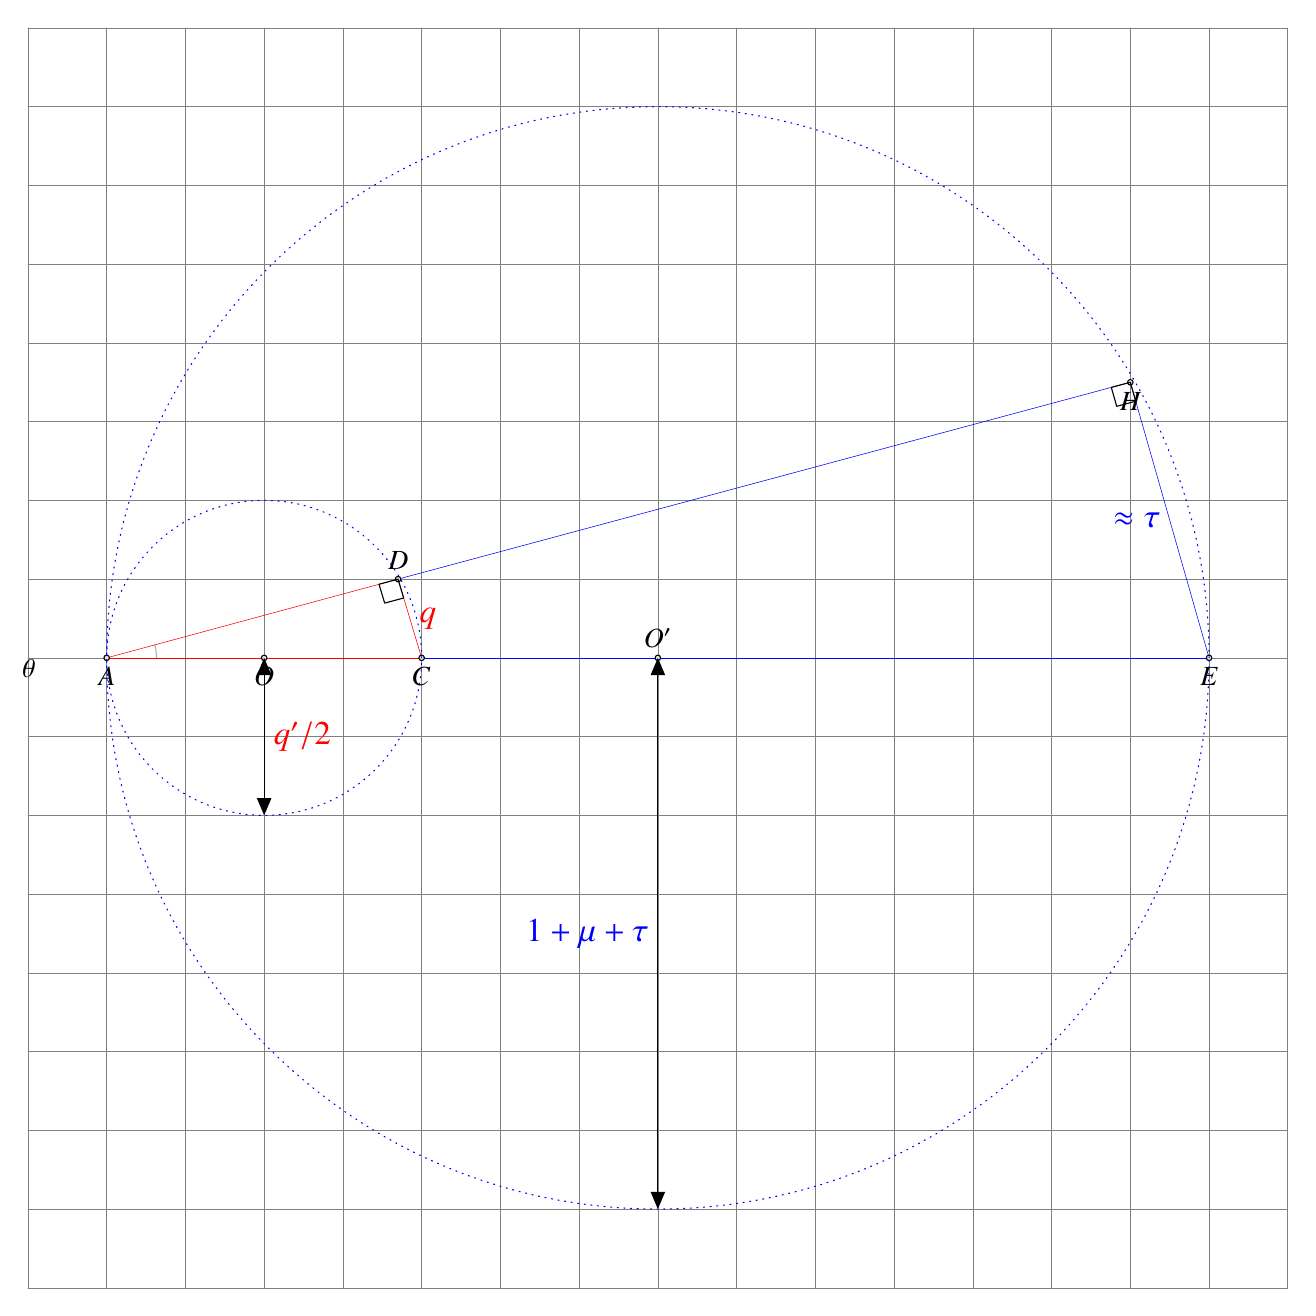
\begin{tikzpicture}[scale=1.0,line cap=round,line join=round,>=triangle 
45,x=1.0cm,y=1.0cm]
\draw[step=1cm,gray,very thin] (-5,-8) grid (11,8);
\tkzDefPoint(-4.,0.){A} 
\tkzDefPoint(0.,0.){C}
\tkzDefPoint(3.,0.){O'}
\tkzDefPoint(10.,0.){E}
\tkzDefMidPoint(A,C) \tkzGetPoint{O}
\tkzInterLC[R](A,C)(C,-0.3cm) \tkzGetSecondPoint{B}
\tkzInterLC[R](C,E)(E,-1cm) \tkzGetSecondPoint{F}
%\tkzDefLine[orthogonal=through D](A,D)
\tkzDefLine[perpendicular=through F](O',E) \tkzGetPoint{G}
\tkzDefLine[perpendicular=through B](O,C) \tkzGetPoint{J}
\tkzDefMidPoint(F,G) \tkzGetPoint{H}
\tkzDefMidPoint(J,B) \tkzGetPoint{D}
%\tkzInterLC(D,tkzPointResult)(O,A) \tkzGetSecondPoint{C}
%\tkzInterLC(F,tkzPointResult)(B,E) \tkzGetSecondPoint{G}
%\tkzDrawPolygon(A,E,H)
\tkzDrawSegment[color=blue](H,E)
\tkzDrawSegment[color=blue](H,D)
\tkzDrawSegment[color=blue](C,E)
\tkzDrawSegment[color=red](A,C)
\tkzDrawSegment[color=red](D,A)
\tkzDrawSegment[color=red](C,D)
\tkzDrawPoints(A,C,D,O,O',E,H)
\tkzLabelPoints(A,C,O,E,H)
\tkzLabelPoints[above](O',D)
%\tkzLabelPoints[left](D)
\coordinate (center) at (O);
\coordinate (center1) at (O');
\draw[blue, dotted]
      let \p1 =  ($(C)-(center)$),
          \n0 = {veclen(\x1,\y1)}
      in (center) circle(\n0);
\draw[blue, dotted]
      let \p1 =  ($(E)-(center1)$),
          \n0 = {veclen(\x1,\y1)}
      in (center1) circle(\n0);
%\draw [<->] (-1.8,1.7) node[right]{} -- (O) node[left]{};
\node [anchor = east,text=blue] at (3.,-3.5) {\large $1+\mu+\tau$};
\draw [<->] (O') node[left]{} -- (3.,-7.) node[right]{};
\node [anchor = west,text=red] at (-2.,-1.) {\large $q'/2$};
\draw [<->] (O) node[left]{} -- (-2.,-2.) node[right]{};
\tkzMarkRightAngle(A,H,E)
\tkzMarkRightAngle(A,D,C)
\tkzDefMidPoint(H,E) \tkzGetPoint{I}
\tkzLabelSegment[left,text=blue](H,E){\large $\approx \tau$}
\tkzLabelSegment[right,text=red](D,C){\large $q$}
%\tkzMarkAngle[fill=blue!20,size=0.4cm,opacity=.5](E,A,H)
%\tkzLabelAngle[pos=1.4](E,A,H){$\theta$}
    \begin{pgfinterruptboundingbox}
        \tkzMarkAngle[fill = gray, size=0.633cm, opacity = .3](C,A,D)
        \tkzLabelAngle[pos = 1.](D,A,C){$\theta$}
    \end{pgfinterruptboundingbox}
\end{tikzpicture}
\caption[Weinberg-Koide Circles]{Weinberg-Koide similitude circles. Figure not drawn to scale.}
\end{figure}






\section {Le modèle électro-faible }
Le modèle standard de la physique des particules a unifié les forces électriques et nucléaires faibles dans le modèle "électrofaible". La théorie de jauge invoquée \cite{Taylor},introduit les charges de jauge {$q'$} (groupe SU(2)) et {$q''$} (groupe U(1)), reliés à la constante électrique $q$ par :

\begin{equation}
 1/q^2 = 1/{q'}^2  + 1/{q''}^2 
 \end{equation}
La notation officielle $g$, {$g’$} est moins symétrique.
la théorie prévoit un photon de masse nulle et trois bosons massifs $W_{+}$, $W_{-}$ et $Z$, caractérisés par un angle de couplage $\theta$  défini par:
\begin{equation}
\cos\theta = m_W/m_Z 
 \end{equation}
et la charge électrique est:
\begin{equation}
q = {q'} \sin\theta = {q''} \cos\theta 
 \end{equation}
 
 
 
 

\begin{figure}
\centering
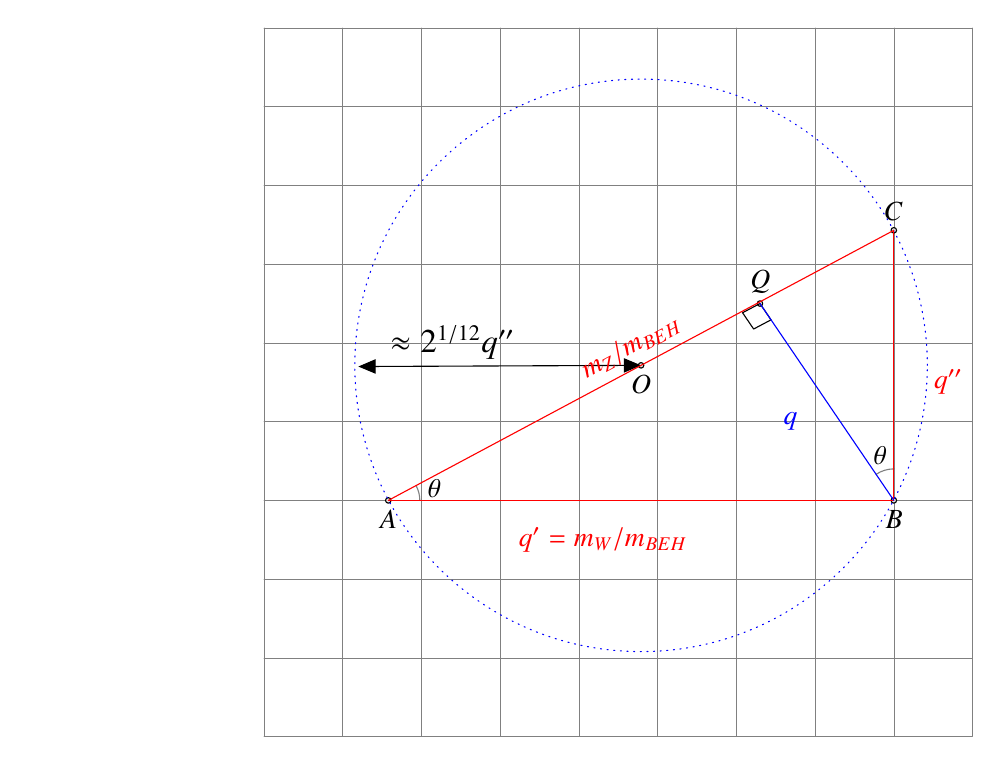
\begin{tikzpicture}[scale=1.0,line cap=round,line join=round,>=triangle 
45,x=1.0cm,y=1.0cm]
%\label{tab:14:table14}
\draw[step=1cm,gray,very thin] (-3,-3) grid (6,6);
\tkzDefPoint(-1.42,0.0){A} \tkzDefPoint(5.,3.43){C} \tkzDefPoint(5.,0.){B} \tkzDefPoint(3.3,2.5){Q}
\tkzDrawPoints(A,C,B,Q)
\tkzMarkRightAngle(A,Q,B)
\tkzLabelPoints[below](A,B)
\tkzLabelPoints[above](C,Q)
\tkzMarkAngle[fill=blue!20,size=0.4cm,opacity=.5](B,A,C)
\tkzLabelAngle[pos=0.6](B,A,C){$\theta$}
\tkzDefMidPoint(A,C) \tkzGetPoint{O}
\coordinate (center) at (O);
\tkzLabelPoints[below](O)
\tkzDrawPoints(O)
\draw [<->] (-1.8,1.7) node[right]{} -- (O) node[left]{};
\tkzLabelSegment[sloped,right,above,text=red](A,C){$m_Z/m_{BEH}$}
\draw[blue, dotted]
      let \p1 =  ($(C)-(center)$),
          \n0 = {veclen(\x1,\y1)}
      in (center) circle(\n0);
\tkzMarkAngle[fill=blue!20,size=0.4cm,opacity=.5](C,B,Q)
%\tkzMarkAngle[fill=blue!20,size=0.4cm,opacity=.5](O,E,D')
\tkzLabelAngle[pos=0.6](C,B,Q){$\theta$}
\draw[color=red] (-1.42,0.) -- (5.,0.);
\draw[color=red] (5.,0.) -- (5.,3.43);
\draw[color=red] (-1.42,0.) -- (5.,3.43);
\draw[color=blue] (5.,0.) -- (3.3,2.5);
\node [anchor = east,text=blue] at (3.9,1.0) {$q$};
\node [anchor = east,text=red] at (6.,1.5) {$q''$};
\node [anchor = east,text=red] at (2.5,-0.5) {$q'=m_W/m_{BEH}$};
\clip(-6.,-0.4) rectangle (0.4,3.4);
\draw[color=black] (-0.5,2.0) node {\large $\approx 2^{1/12} q'' ~~$};
\end{tikzpicture}
\caption[Weinberg Triangle]{Weinberg Triangle.}
\end{figure}





 
 
 \begin{figure}
\centering
\begin{tikzpicture}[scale=0.75]
%\tkzInit[xmax=6.4, zmax=3.4]
\tkzDefPoint(0.0,0.0){A} \tkzDefPoint(6.4,0.0){B} \tkzDefPoint(5.1,-1.3){C} \tkzDefPoint(4.0,-1.0){q}
\tkzDrawPoints(A,B,C,q)
\tkzDefMidPoint(B,q) \tkzGetPoint{D}
%\tkzDefPoint[label={[align=left]right:$q$},xshift=00mm](4.5,-0.5){D}
\tkzLabelSegment[sloped,text=red,xshift=-06mm](q,B){$q$}
\tkzMarkRightAngle(A,B,C)
\tkzMarkRightAngle(B,q,C)
\tkzLabelPoints[below](A,B,C)
%\tkzLabelPoints[above right](q)
\tkzMarkAngle[fill=blue!40,size=1.4cm,opacity=.5](C,A,B)
\tkzLabelAngle[pos=1.6](C,A,B){$\theta$}
    %\draw [important line] (0.0,0.) coordinate (A) -- (5.1,-1.3) coordinate (C) node[below, text width=5em] {}
    %\draw [blue] (6.4,0.) coordinate (A) -- (4.,-1.0) coordinate (D) node[below, text width=5em] {$h$}
    %\draw [red] (6.4,0.) coordinate (B) -- (4.,-1.0) coordinate (D) node[below, text width=5em] {$q$}
  \draw (6.4,0,0) coordinate (x) |- (0,10,0) coordinate [midway] (h) coordinate (y) -- (0,10,3.4) coordinate (a) -- (0,0,3.4) coordinate (z) -- (6.4,0,3.4) edge (x) -- (6.4,10,3.4) coordinate (v) edge (h)
  -- (a)  ;
  \draw [dashed] (0,0,0) coordinate (o) edge (x) edge (y) -- (z);
  \draw [dashed] (0,0,0) coordinate (o) edge (x) edge (v) -- (v);
  \draw [blue] (0,0,0)  -- (6.4,0.0,3.4);
  \draw [red] (4.9,0.02,2.7)  -- (6.4,0.0,0.0);
  %\node [circle, minimum size=2pt, inner sep=0pt, fill, label=135:$\sqrt{2a^3/pp_G}$] at (v) {};
  \draw [very thin,black,line join=round] (0,0,0)  -- node [sloped,above] {$\sqrt{2a^3/pp_G}$} (6.4,10,3.4);
  \node [circle, minimum size=4pt, inner sep=0pt, fill, label=135:o] at (o) {};
  \draw [decoration={markings,mark=at position 1 with
    {\arrow[scale=3,>=stealth]{>}}},postaction={decorate}] (0,0,0) -- (6.4,10,3.4);
  \draw [dashed] (0,0,0) -- (6.4,0,3.4);
  \draw [->] (x) -- +(3pt,0,0) node [midway,above] {$q'$};
  \draw [->] (y) -- +(0,3pt,0) node [midway,right] {$1$};
  \draw [->] (z) -- +(0,0,3pt) node [midway,above] {$q''$};
  %\draw (v) -- ++(0,0,-2) coordinate (d) -- ++(-2,0,0) coordinate (e) -- ++(0,0,2) |- ++(2,-2,0) coordinate [midway] (f) -- ++(0,0,-2) coordinate (g) -- (d);
  %\draw [dashed] (e) -- ++(0,-2,0) coordinate (c) edge (f) -- (g);
  %\node [label=45:C] at (c) {};
  %\draw[red]   (0,0,0) -- (.95,0,0)    node[red,left=6pt]    {$x$};
\end{tikzpicture}
\caption[The Weinberg-Sanchez cuboid]{3D perspective of the "Weinberg-Sanchez" cuboid: Electro-weak / Gravitation connection}
\end{figure}
















\begin{figure}
\centering
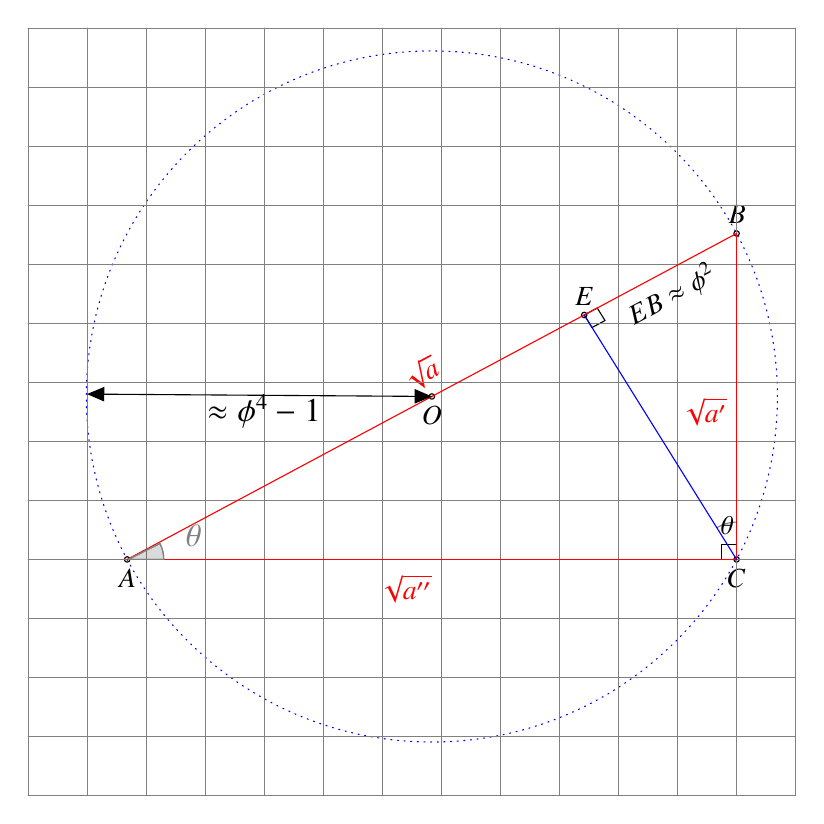
\begin{tikzpicture}[scale=0.75,line cap=round,line join=round,>=triangle 
45,x=1.0cm,y=1.0cm]
%\label{tab:13:table13}
\tkzDefPoint(-4.32,0.0){A} \tkzDefPoint(6.0,5.52){B} \tkzDefPoint(6.,0.){C} %\tkzDefPoint(0.0,0.0){D}
\tkzDrawPoints(A,B,C)
\tkzMarkRightAngle(B,C,A)
%\tkzMarkRightAngle(B,D,C)

\tkzLabelPoints[below](A,C)
\tkzLabelPoints[above](B)
\tkzDefMidPoint(A,B) \tkzGetPoint{O}
\coordinate (center) at (O);
\tkzLabelPoints[below](O)
\tkzDrawPoints(O)
%\tkzDefInterPoint(A,C) \tkzGetPoint{O}
\tkzLabelSegment[sloped,above,text=red](A,B){$\sqrt{a}$}
\draw[blue, dotted]
      let \p1 =  ($(-4.32,0)-(center)$),
          \n0 = {veclen(\x1,\y1)}
      in (center) circle(\n0);
\tkzDefMidPoint(O,B) \tkzGetPoint{E}
\tkzDrawPoints(E)
\tkzLabelPoints[above](E)
\tkzMarkRightAngle(B,E,C)
\draw[step=1cm,gray,very thin] (-6,-4) grid (7,9);
\draw[color=red] (-4.32,0.) -- (6.,0.);
\draw[color=red] (6.,0.) -- (6.,5.52);
\draw[color=red] (-4.32,0.) -- (6.,5.52);
\draw[color=blue] (E) -- (C);
\tkzDefMidPoint(E,B) \tkzGetPoint{F}
\tkzLabelSegment[sloped,below,text=black](E,B){$EB \approx \phi^{2}$}
\tkzMarkAngle[fill=blue!20,size=0.633cm,opacity=.5](B,C,E)
\tkzLabelAngle[pos=0.6](B,C,E){$\theta$}
%\node [anchor = east] at (1.,3.5) {$\sqrt{a}$};
\node [anchor = east,text=red] at (6.,2.5) {$\sqrt{a'}$};
\node [anchor = east,text=red] at (1.,-0.5) {$\sqrt{a''}$};
\draw [<->] (O) node[left]{} -- (-5.0,2.8) node[right]{};
\clip(-6.,-0.4) rectangle (0.4,3.4);
\draw [shift={(-4.3,0.)},color=gray,fill=darkgray,fill opacity=0.1] (0,0) -- (0.:0.6) arc (0.:26.9:0.6) -- cycle;
\draw [shift={(-4.3,0.)},color=gray,fill=darkgray,fill opacity=0.1] (0,0) -- (0.:0.6) arc (0.:26.9:0.6) -- cycle;
%\draw[color=gray,fill=darkgray,fill opacity=0.1] (0.,0.42) -- (-0.42,0.42) -- (-0.42,0.) -- (0.,0.) -- cycle; 
%\draw (0.,6.)-- (-4.32,0.);
%\draw (6.,5.52)-- (-4.32,0.);
%\draw (6.,0.)-- (6.,5.52);
\draw[color=gray] (-3.2,0.4) node {\large $\theta$};
\draw[color=black] (-2.,2.5) node {\large $\approx \phi^4-1$};
\draw[color=gray] (0.34,0.33);
%\tkzMarkRightAngle[fill=blue!20](B,F,C)
\end{tikzpicture}
\caption[Electric Triangle properties]{Electric Triangle.}
\end{figure}



\section {Le boson scalaire massif et la relation gravito-électrofaible }
Les masses des bosons W et Z sont reliées à la masse du boson scalaire massif (Brout-englert-Higgs), voir le triangle de Weinberg (Fig). En le complétant par un troisième axe portant l'unité, on obtient un vecteur de module directement lié à la constante holique ci-dessus, où $H$ est remplacé par la masse gravitationnelle du proton gravitationnelle $p_G$ ci-dessus:

\begin{equation}
 1 + {q'}^2  + {q''}^2 = 1 + (m_Z/m_{BEH})^2 \approx 2a^3/pp_G = 2m_N^3\sqrt{N_L}/m_Pm_em_p
 \end{equation}
 
où $m_P$ est la masse de Planck. Avec la valeur du boson scalaire $ m_{BEH} = 495^2 m_e $, on obtient une valeur de $m_Z$ à $10^{-7}$ de la valeur précédemment optimisée  \cite{Sanchez2} (table 1). 




\section{La relation avec le couplage électrique}
La relation entre la charge électrique adimensonnelle $q$ et le couplage électrique $a$ est \cite{Taylor}
\begin{equation}
 a/4 \pi = 1/q^2 = 1/{q'}^2  + 1/{q''}^2 
 \end{equation}
 
 
  Cela correspond aux paramètres numériques:
\begin{equation}
 4\pi / {q'}^2  = {a'}  \approx 30 ,    ~~~~         4\pi / {q''}^2  = {a''}  \approx 107
 \end{equation}
 
c'est-à-dire:
\begin{equation}
\sqrt{a}  = \sqrt({a'} + {a''}) = \sqrt{a'} / \sin\theta  = \sqrt{a''}  / \cos\theta
 \end{equation}


Ces relations sont illustrées dans le « triangle électrique » fig.3.

La charge électrique $q = \sqrt{4\pi/a} $ montre une connection avec la forme trigonométrique \cite{Sanchez2} $a \approx 44\pi - Arccos(1/e)$

\begin{equation}
a \approx 44\pi_a + ln(\sqrt {4\pi_a/a})     ~~~~ \rightarrow 6\pi_a^5 \approx p ~~~~ \pi_a : 3, 7, e^e + 1
 \end{equation}

Ainsi la charge électrique $q$  est intimement relié au couplage électrique $\sqrt a$. Le triangle représentatif de ce dernier montre une nette connexion avec les puissances 2 et 4 du nombre d'or, dont la pertinence avait été prédite \cite{Sanchez1}.







 
 
 
 
 
 
 
 
 
 
 
 
 
 
 
 
 
 






\section{Connexions avec le générateur de Lucas-Lehmer}

Le générateur de Lucas-Lehmer est le nombre $(2 + \sqrt 3)$, lié à $a$ et $a^a$, ce dernier terme étant aussi lié au générateur de Pell-Fermat $(1 + \sqrt2)$. Les puissances de type $2^n$ de ce générateur produisent des nombres dont la partie entière est la série de Lucas-Lehmer, qui permet de déterminer si un nombre de type Mersenne $2^n-1$ est premier. Ce générateur se caractérise par:


\begin{equation}
(2 + \sqrt 3) + 1/ (2 + \sqrt 3) = 4
\end{equation}


On observe, à 20 ppb:

\begin{equation}
(2cotg\theta) + 1/(2cotg\theta) \approx \sqrt(4^2 + 1/5^2)
\end{equation}

ce qui semble impliquer l'espace 5D prévu par Eddington, en réinterprétant l'algèbre de Dirac.

De plus, on observe la connexion suivante impliquant la fonction topologique $f(d) = exp(2^{d/4})$ et $136$, la première estimation
d'Eddington pour $a$:

\begin{equation}
(q\cos\theta + 1/q\cos\theta )/4 \approx f(-a/4d_e)    \approx (2(a-136))^{1/(2\times 137)}
\end{equation}

tandis que:

\begin{equation}
 1/q\cos\theta \approx e^{2a /(\mu+1)}    \approx (2+\sqrt3)(2a^3p/H^2n)^{1/a}
\end{equation}

de sorte qu'on retrouve un terme analogue à la racine holique ci-dessus du rayon de Hubble. 

\textit{La tryptique $136-137-a$ est vraiment au centre de l'Arithmétique Cosmique}












%une interaction entre la matrice d’espace-temps $4 \times 4$ et la matrice $5 \times 5$. The later was indeed predicted by Eddington, who showed that the Dirac algebra corresponds to a five-dimensional base space. 


En effet, d'après Salingaros \cite{Salingaros}: \textit{Indeed, it seems that Eddington was really ahead of his time : Eddington anticipated results of current interest. He discovered the Majorana spinors, and was responsible for the standard $\gamma^5$ notation as well as the notion of chirality. Furthermore, Eddington defined Clifford algebras in eight and nine dimensions which are now appearing in grand unified gauge and supersymmetric theories. A point which Eddington cleared up, yet is still misunderstood, is that the Dirac algebra corresponds to a five-dimensional base space.}


La pertinence de l'exposant $a$ est confirmé par la triple relation suivante (écarts -1.69, -1.73 et 0.01 $\times 10^{-3}$, impliquant le nombre "économique" géant  $ E = exp(exp(e^e))$:

\begin{equation}
  P^4  \approx E^{1/(a-1)^2} \approx (9/2)^a \approx (1/\sin theta)^{ja}/d_e^4 
\end{equation}

où $j = 2d_e$ est le moment magnétique de l'électron.







\section{La connexion avec la table périodique des élements chimiques}

Les dimensionalités de la série anormale des cordes $d = 2 + 4k$, qui apparaissent dans l’Axe Topologique  sont les nombres $2, 6, 10, 14, 18, 22, 26, 30$. Les quatre premiers s’identifient avec les nombres atomiques de la série spectroscopique s,p,d,f. La table périodique contient 19 de ces séries, aboutissant à l’Oganesson, de numéro atomique $7s + 6p + 6d + 2f = 118$. Mais les périodes se distinguent des nombres quantiques principaux, de telle façon que les périodes, à partir de la deuxième, sont doubles, de sorte que le nombre ci-dessus se décompose en $118/2 = 59 =  1+3s+3p+2d+f$. En séparant les termes extremes $f + 1 = 15$, la séparation théorique $137 = 107 + 30$ est justifiée par la somme $137 = 7(s+1)+6(p+1)+4(d+1)+2(f+1)$.



\section{Retour sur les quatre algèbres principales}

Le pythagorisme s’accorde avec la nature quantique du monde, en particulier les nombres quantiques de la physique des paticules. Ainsi le nombre 30 n’est pas neutre. C’est non seulement la dimensionalité terminale de l’axe topologique, mais aussi le seul cas où l’aire d’ un triangle de Pythagore (12,5,13) est égal à son périmètre.  Il peut être considéré comme le produit des trois dimensionnalités basiques, $2 \times 3 \times5$. La triade suivante de nombres premiers est le produit $3 \times 5 \times7 $ = 105, de sorte que la formule de base serait:


\begin{equation}
30 + 105 = 135 = 5 \times 3^3
\end{equation}

Où $5$ et $3^3$ sont les deux premiers nombres co-parfaits, précédant 495. Si on rétablit l’algèbre des nombres complexes qu’Atiyah avait ôté de la série, on aboutit au nombre 139, la partie entière de $a_{00} = i^{\pi/i} = e^{\pi^2/2}$. \textit{Il apparaît que 137 est la moyenne de ces deux nombres}. 

\section{Conclusion}

Le propre de la Science est que l’on peut progresser sans connaître la théorie ultime, par approximations successives.  La non-reconnaissance de cette évidence historique a fait rejeter plusieurs théories et formules empiriques que le principe de rationalisation symbolique de $\pi$ réhabilite pleinement. Contrairement à la tendance actuelle de formalisation à outrance, les mathématiques doivent maintenant s’apuyer sur la physique de précision pour se compléter. 






\begin{table}
\caption{Adimensional primary constants}
%% \label{tab:1}
\label{tab:1:table1}
  \hskip-2.0cm\begin{tabular}{llll}
    \toprule
    %\multicolumn{4}{c}{}                   \\
    \cmidrule(r){1-4}
    name & symbol    & value & imp (ppb) \\
    \midrule
    
    Euler-Napier constant  & e    & 2.718281828459042 & "exact" \\    
    Archimedes constant & $\pi$    & 3.14159265358979 & "exact" \\    
    $\pi$ fifth fractional term & $\pi_5$    & 292.63459101440 & "exact" \\ 
    Euler-Mascheroni constant & $\gamma$    & 0.57721566490153 & "exact" \\    
    
     
    Electric constant  & $a_{mes}$    & 137.035999084(21) & 0.15 \\
    Excess Electron Magnetic moment  & $d_e$    & 1.00115965218128 & 0.15 \\
    Measured massive scalar boson/Electron mass ratio  & $H^0_{meas}$ & 245000(250)  & $10^6$ \\
    Optimized massive scalar boson/Electron mass ratio  & $H^0$ & $ 495^2 = 245025$  & exact \\
    
    Measured W boson/Electron mass ratio  & $W_{meas}$ & 157297(24)  & $1.5 \times 10^5$ \\     
    Optimized  W boson/Electron mass ratio  & $W$ & 157340.1093  & ppb\cite{Sanchez2} \\     
    This work  W boson/Electron mass ratio  & $W$ & 157340.1100  & ppb \\
    
    Measured Z boson/Electron mass ratio  & $Z_{meas}$ & 178450(4)  & $2.3 \times 10^4$ \\     
    Optimized  Z boson/Electron mass ratio  & $Z$ & 178451.7402  & ppb\cite{Sanchez2}\\     
   This work  Z boson/Electron mass ratio  & $Z$ & 178451.7171  & ppb\\
   
  Effective "weak-mixing angle"  & $(\sin \theta)^2(m_Z)$    & 0.23155(4) & $1.7 \times 10^7$ \\
  This work "weak-mixing angle" & $(\sin \theta)^2(m_Z)$    & 0.231475 &  \\
  
   Optimized SU(2) coupling &{$q'$}     & 0.6421390034 & 0.15 \\
   Optimized U(1) gauge coupling & {$q''$}    & 0.3436256462 & 0.15 \\
   Optimized electric charge & $ q $    & 0.302973211 & 0.15 \\
        
    Atiyah constant & $\Gamma$    & 25.17809724196  & 0.15 \\                  
    Lucas Large Prime Number & $N_L$    & $2^{127}-1$  & exact \\     
    Measured Fermi/Electron $m_F/m_e$ & $F_{meas}$   & 573007.362  & 250 \\ 
    Fermi Sanchez-Atiyah mass ratio: & $F$   & 573007.3652  & 0.22 \\      
    Proton/Electron mass ratio $m_p/m_e$ & p   & 1836.15267343  & 0.06 \\  
    Hydrogen/Electron mass ratio  & $H$  & 1837.15266014  & 0.06 \\      
    Neutron/Electron mass ratio  & $n$ & 1838.6836617  & 0.5 \\     
    Measured Muon/Electron mass ratio  & $\mu_{meas}$ & 206.7682830  & 22 \\     
    Optimized Muon/Electron mass ratio  & $\mu$ & 203.7682869  & 0.1 \\     
    Measured Tau/Electron mass ratio  & $\tau_{meas}$ & 3477(2)  & $7\times 10^4$ \\        
    Optimized Koide Tau/Electron mass ratio  & $\tau$ & 3477.441701  & 0.1 \\  
 
 Planck ratio $m_P/m_e$ & P   & $2.389015907 \times 10^{22}$ &ppb  \cite{Sanchez2}  \\
 Gravitational proton ratio $P N_L^{-1/2}$ & $p_G$    & $ 1831.531181 $ &ppb  \cite{Sanchez2}  \\
 Gravitational coupling constant $R/2\lambdabar_e = P^2/pH$ & $a_G$   & $1.691936467 \times 10^{38}$ &ppb  \cite{Sanchez2}  \\
 Electroweak coupling constant $F^2 = (2\gamma\times 137)^3$ & $a_w$     & $3.283374406 \times 10^{11}$ & ppb \cite{Sanchez2}  \\
Optimised Strong coupling constant $a_w/2\pi(pH)^{3/2}$ & $a_s$   & $8.434502906$ & ppb \cite{Sanchez2} \\
  
    
         
   \bottomrule
  \end{tabular}
\end{table}



\begin{table}
\caption{Physical constants}
\label{tab:2:table2}
  \hskip-2.0cm\begin{tabular}{lllll}
    \toprule
    %\multicolumn{5}{c}{}                  \\
    \cmidrule(r){1-5}
    \ name & Symbol  & unit  & Value & imp (ppb) \\
    \midrule
  
 Relativity speed     & c   & $m s^{-1}$   & 299792428 & exact \\
 Planck constant     & h   & J s   & $6.62607015 \times 10^{-34}$ & exact \\
 Reduced Planck constant $h/2\pi$    & $\hbar$   & J s   & $1.05457181 \times 10^{-34}$ & "exact" \\
 Official Gravitation constant   & $G_{off}$ & $kg^{-1} m^3 s^{-1}$ & $6.67430 \times 10^{-11}$  &  contested\\
 Optimized Gravitation constant   & G & $kg^{-1} m^3 s^{-1}$  & $6.67545375\times 10^{-11}$  &  ppb \cite{Sanchez2} \\
 Fermi constant  & $G_F$ & $J m^3$   & $61.435851 \times 10^{-62}$  &  500\\
 Electron mass $m_e = m_p/p = m_H/H = m_n/n$  & $m_e$ & kg  & $9.1093837015 \times 10^{-31}$  &  0.3\\
 
 
 
 Electron reduced wavelength $\hbar/m_ec$ & $\lambdabar_e$ &  m   & $3.861592675\times 10^{-13}$  & 0.3\\
 Electron classical radius $\hbar/am_ec$ & $r_e$ &  m   & $2.817940322\times 10^{-15}$  & 0.45\\
 Hydrogen Bohr radius $a(1+1/p)\lambdabar_e$ & $r_H$ &  m   & $5.294654092 \times 10^{-15}$  & 0.45\\
 Proton radius  & $r_p$ &  m   & $8.8\times 10^{-16}$  & contested\\
 Planck length $(\hbar G /c^3)^{1/2}$ & $l_P$  & m  & $1.61639471 \times 10^{-35}$ & ppb \cite{Sanchez2}  \\
 
 Rydbergh reduced wavelength $\lambdabar_e(2aH/p)^2$ & $\lambdabar_{Ryd}$  & m  & $1.45190673 \times 10^{-8} $ & 0.3   \\
 

    \bottomrule
  \end{tabular}
  % \label{tab2:table2}
\end{table}



\section {Acknowledgements}

The authors thank Anatole Khelif for many thoroughful discussions, including with Atiyah, and Denis Gayral for technical assistance.

\bibliographystyle{unsrt}  
%\bibliography{references}  %%% Remove comment to use the external .bib file (using bibtex).
%%% and comment out the ``thebibliography'' section.
%%% Comment out this section when you \bibliography{references} is enabled.
\begin{thebibliography}{99}

\bibitem{Tanabashi} Tanabashi M. et al. (Particle Data Group), Phys. Rev. D98, 030001 (2018), and 2019 update.\\

\bibitem{Sanchez1}  Sanchez F.M., Holic Principle, Entelechies, ANPA 16, Sept. 1995. Bowden K.G., 324--343.\\

\bibitem{Sanchez2} F.M. Sanchez, V. Kotov, M. Grosmann, D. Weigel, R. Veysseyre, C. Bizouard, N. Flawisky, D. Gayral, L. Gueroult, ``Back to Cosmos''. Progress in Physics, vol. 15, issue 2, (2019). http://www.ptep-online.com/2019/PP-57-12.PDF .\\


\bibitem{Hooft}  Hooft, Nucl.Phys. B 335, 138, (1990); L. Susskind, J. Math. Phys. 36, 6377 (1995) ; arXiv:hep-th/9409089\\

\bibitem{Seiberg} Emergent Spacetime. The Quantum Structure of Space and Time, Proccedings of the 23rd Sovay Conference on Physics, Brussels, Belgium, ed. David Gross, Marc Henneaux and Alexander Sevrin, World Scientific, Dec. 2005, 163-178.\\


\bibitem{Weigel} Veysseyre R., Veysseyre H., and Weigel D. "Counting, types and symbols of crystallographic Point Symmetry Operations of space E^{n}" AAECC 5, 53--70 (1992) DOI: 10.1007/BF01196625 ISBN: 0938-1279.\\

\bibitem{Veysseyre} Veysseyre R., Veysseyre H., and Weigel D. "Nombre de types d’opérations ponctuelles de symétrie cristallographiques dans l’espace E^{n} . (Number of types of crystallographic point symmetry operations of space E^{n} )", Comptes Rendus de l’Académie des Sciences. Série II (Jan.1990).\\

\bibitem{Wyler} Wyler A., "L'espace symetrique du groupe des equations de Maxwell" C. R. Acad. Sc. Paris, t. 269, 743-745 (1969). Wyler A., C.R. Acad. Sci, Paris "Les groupes des potentiels de Coulomb et de Yukawa". C. R. Acad. Sc. Paris, t. 272, 186-188 (1971).\\

\bibitem{Atiyah} Atiyah M. Heidelberg Laureate Forum 24th Sept 2018 https://hitsmediaweb.h-its.org/Mediasite/Play/35600dda1dec419cb4e99f706197a3951d. \\ 

\bibitem{Green} Green, M. Schwarz J. (1984)  Anomaly cancellations in supersymmetric D = 10 gauge theory and superstring theory". Physics Letters B. 149: 117.\\



\bibitem{Friedman} Friedman W. et al, The Carnegie-Chicago Hubble Program. VIII. An Independent Determination of the Hubble Constant Based on the Tip of the Red Giant Branch, arxiv : 1907.05922.\\

\bibitem{Eddington} Eddington A, ``Fundamental Theory'', Cambridge University Press (1949).\\

\bibitem{Bekenstein} Bekenstein J. ``Black holes and entropy'', Phys. Rev. D 7:2333-2346 Issue:8. DOI:10.1103/PhysRevD.7.2333 (1973) \\

\bibitem{Quinn} Quinn T, Speake C, Parks H, Davis R. 2014 The BIPM measurements of the Newtonian constant of gravitation, G. Phil.Trans. R. Soc. A372: 20140032. https://royalsocietypublishing.org/doi/10.1098/rsta.2014.0032 \\

\bibitem{Sternheimer} Sternheimer J., Musique des particules elementaires, CRAS, 297, II, 829--834 (1983).\\

\bibitem{Bastin} Bastin T. and Kilmister C.W., Combinatorial Physics (World Scientific, 1995).\\

\bibitem{Koide} Koide Y., Fermion-Boson Two-Body Model of Quarks and Leptons and Cabibbo Mixing  Lett. Nuovo Cimento 34, 201 (1982).\\

\bibitem{Salingaros} Salingaros N., Some Remarks on the Algebra of Eddington's E Numbers. Foundations of Physics, June 1985, Volume 15, 6, pp 683–691.\\

\bibitem{Taylor} Taylor John G., "The New Physics", American Journal of Physics, Vol.41, p 1381--1382, DEC.1973,doi: 10.1119/1.1987588


\end{thebibliography}








\begin{table}
\caption{15 ppb precise formula for $R \approx 13.8119768$ Gly}
\label{tab:8:table8}
  \hskip-2.0cm\begin{tabular}{llll}
    \toprule
    \multicolumn{3}{c}{}                   \\
    \cmidrule(r){1-3}
    \#     & Formula  & Remarks \\
    \midrule
 
 
 15 &  $(2\pi_R a^3)^5 \lambdabar_{e}^2/6\lambdabar_H  $ &  $\pi_{R} = 3+1/(7 + 1/(16 + 2/e^{2e})$  \\ 
 
  14 & 2 $\lambdabar_{e} (a/137) (p/6) (pH)^6\pi_{synth}^5= /a_s (1+a^2/F) $ & Eddington's Eq 4 coupling forces:  $\pi_{synth} = 3+1/(7 + 1/(16 -(a-137) +2/a_s\pi_5$  \\ 
        
 
  13 & $ 8\pi l_P (R_N/\lambda_{CW})^2 (\sqrt{(137^2 + 1/4 + 2/127)}/\pi^{2/3})   $ & confirms the Cosmos temperature   \\  
   
    12 & $ 8\pi l_P (R_N/\lambda_{CW})^2 (137/\pi_0)^{1/3}   $ & with $\pi0 = 3+1/(7+1/(16+1/12^2))$ confirms the Atiyah's symmetry $a--\pi$    \\
  
   11 & $(6p_W/5p)\lambdabar_{e} a^{16 \sqrt a_s} e^{-1/f(10)}$ & from the Cosmos radius $R_C$ with $\pi_{44\pi} = 3+1/(7 + 1/(16 + 1/3\sqrt{44\pi})$  \\
  
   10 & $\lambdabar_{e} ((44\pi_{44\pi} -a) R_C^{1/(1+ a^{1/2} /e^2)}$ & from the Cosmos radius $R_C$ with $\pi_{44\pi} = 3+1/(7 + 1/(16 + 1/3\sqrt{44\pi})$  \\ 
        
     9 & $ \lambdabar_{e} (3^3)^{3^3} e^{\pi_1^2/2}/139  $ & from the Cosmos holographic radius $R_N$ with $\pi_1 = 3+1/(7 + \beta a/137\times 16$  \\
    
            
     8 & $ \beta ^(1/4) (2p/H)^4 \lambdabar_{e} \pi_5^{16}/(a_0 - 2) $   & confirms the central role of $\pi_5$ \\
    
      7 & $ \sqrt{137p/an} R_C/P^2 a^6 6\pi_d^5 $   & with $\pi_d = 3 + (1/(7+1/(15 + d_e)))$  \\           
      6 & $2 N_L\lambdabar_{e} a^5((e-\pi/2)/137p_W)^2$   & pertinence of the relation $e \approx \pi/2 + ln\pi$  \\       
     
  
      
      5 & $\lambdabar_{e} g(6)/(1+\sqrt(137^2+\sqrt(136))/jn)$  & Confirms $137=136+1$, with the scale constant $j = 8\pi^2/ln2 $ \\
      4 & $(\lambdabar_{e} 2^{128})(1-(137^2+\pi^2+e^2)/pH)$ & shows a symmetry between $\pi$, e and 137, prolongating $ a \approx (137^2 + \pi^2)^{1/2}$ \\
       3 & $2\lambdabar_{e} (pn/H^{2})(g(5)/\ln(2-1/ja^2))^2$   & confirms the Topological axis $g(5)^2/g(6) = 25/6 \rightarrow \ln(2) \approx 2\sqrt(3/5)$  \\    
      2 & $(\lambdabar_{e} 2^{137})(\gamma^2 n^6 / 137^2 \Gamma^{11})$ & superstring liaison 11D-9D, with $\Gamma$, the Atiyah constant \\
      1 & $(\lambdabar_{e} 2^{128}/d_e^2(m_H/m_p)^6$  & empiric [5], separates the neutron from $\Gamma \gamma^2 d_e^2 \approx (p\Gamma^2 \sqrt(137)/2 \sqrt(2) Hn)^6 \approx a_s$ \\
    
    \bottomrule
  \end{tabular}
\end{table}


% \section{Periodic Table}
%^^^^^^^^^^^^^^^
% \input{periodic-table}



\end{document}





\begin{table}
\caption{Cosmic constants}
\label{tab:3:table3}
  \hskip-2.0cm\begin{tabular}{lllll}
    \toprule
    %\multicolumn{5}{c}{}                   \\ 
      \cmidrule(r){1-5}
     name & Symbol   & unit   & Value & imp (ppb) \\
 \midrule
       
   Official Hubble-Lemaitre so-called "present" constant & $c/H_0$ & Gly & 13.80(2)    & $1.5 \times 10^6$ \\  
   Critical Universal radius $2\hbar^2/Gm_em_pm_H=2GM/c^2=2a_G\lambdabar_{e}$ & R &  Gly & 13.81197677  & this work ppb\\   
   Universal mass $Rc^2/2G = m_P^4/m_em_pm_H$ & M & kg & $8.796524777 \times 10^{52}$ & this work ppb \\    
   Universal energy density & $u_U$ & $J/m^3$ & $8.459065716 \times 10^{-10}$ & this work ppb \\   
   Cosmos hologram Nambu radius & $R_N$ &  m & $1.712894163 \times 10^{26}$ & this work ppb\\   
   Cosmos radius & $R_{GC}$ &  m & $9.075773376 \times 10^{86}$ & this work ppb \\   
   Universal mono-electron radius & $R_1$ &  m & $1.492365473 \times 10^{26}$ & this work ppb \\    
   Official CMB temperature & $T_{CMBoff}$ & K & $2.7255(6)$ & $2 \times 10^5$ \\    
   Cosmos (CMB) temperature & $T_{C}$ & K & $2.725820138$ & this work ppb \\
   Cosmos (CMB) thermal reduced wavelegth & $\lambdabar_{C} = \hbar c/ k_B T_C $ & m & $8.400716621 \times 10^{-4} $ & this work ppb \\ 
   
   Cosmos (CMB) thermal Wien wavelegth & $\lambda_{CW} = \hbar c/ w $ & m & $8.400716621 \times 10^{-4} $ & this work ppb \\ 
   
   
   Neutrino temperature  $(CNB)T_{CMB}/ (4/11)^{1/3}$ & $T_{CNB}$ & K & $1.945597343$ & this work ppb \\ 
   CMB energy density $(\pi^{2/15})\hbar c/ \lambdabar_{CMB}^4 \approx (2a_s^2)^2 u_U$ & $u_{CMB}$ & $J/m^3$ & $4.176762758 \times 10^{-14}$ & this work ppb\\ 
   CMB photon density $16 \pi \zeta (3)/\lambda_{CMB}^3$  & $l_{ph}^{-3}$  & $m^{-3}$   & $410.871743 \times 10^6 m^{-3}$ & this work ppb \\ 
   CNB energy density $u_{CMB} = (3\times (7/8) \times (4/11)^{4/3})$ & $u_{CNB}$ & $J/m^3$ & $2.84572016\times 10^{-14}$ & this work ppb \\  
   Non-Doppler quasar period & $t_{Kmes} = l_K/c$ & sec & 9600.60(1) & 1000 \\  
   Optimized Non-Doppler quasar period $\lambdabar_e (a_Ga_w)^{1/2}/c$ & $t_{K}$ & sec & 9600.591457 & this work ppb \\ 
   Equivalent number of neutrons in the critical sphere & $n_n$ & - & $5.251883912 \times 10^{79}$ & this work ppb \\ 
   Number of photons in the critical sphere  & $n_{ph}$ & - & $3.840045866 \times 10^{87}$ & this work ppb \\ 
   Number of photons in the Cosmos  & $N_{ph}$ & - & exp(621.949984) & this work ppb \\ 
   Equivalent number of Hydrogen atoms in the Cosmos  & $N_H$ & - & exp(603.8432382) & this work ppb \\
 \bottomrule
  \end{tabular}
  % \label{tab3:table3}
\end{table}
 
 
 


\begin{figure}
\centering
\begin{tikzpicture}[scale=1.50, line cap=round,line join=round,>=triangle 
45,x=1.0cm,y=1.0cm]
%\label{tab:15:table15}
\tkzDefPoint(-0.236,0.0){A} \tkzDefPoint(0.0,0.944){B} \tkzDefPoint(3.764,0.){C} \tkzDefPoint(0.0,0.0){D} \tkzDefPoint(0.882,0.0){D'} \tkzDefPoint(0.882,-1.764){E}
\tkzDrawPoints(A,B,C,D,D',E)
\tkzMarkRightAngle(A,B,C)
\tkzMarkRightAngle(B,D,C)
\tkzMarkRightAngle(E,D',C)
\tkzMarkRightAngle(A,E,C)
\tkzLabelPoints[below](A,C,D,E)
\tkzLabelPoints[above](B,D')
\tkzDefMidPoint(A,C) \tkzGetPoint{O}
\coordinate (center) at (O);
\tkzLabelPoints[below](O)
\tkzDrawPoints(O)
\tkzMarkAngle[fill=blue!20,size=0.4cm,opacity=.5](B,O,D)
%\tkzMarkAngle[fill=blue!20,size=0.4cm,opacity=.5](O,E,D')
\tkzLabelAngle[pos=0.6](B,O,D){$\theta$}
\tkzLabelAngle[pos=0.6](O,E,D'){$\theta$}
%\tkzMarkAngle[fill=blue!40,size=1.4cm,opacity=.5](C,A,B)
%\tkzLabelAngle[pos=1.6](C,A,B){$\theta$}
\draw[step=1cm,gray,very thin] (-1,-3) grid (4,3);

\draw[color=green] (-0.236,0.) -- (0.882,-1.764);
%\draw[color=green] (-1.764,0.) -- (0.,0.0);
\draw[color=green] (-0.236,0.) -- (3.826,0.);
\draw[color=green] (0.882,-1.764) -- (3.826,0.);
\draw[color=blue] (0.882,0.) -- (0.882,-1.764);
% 1st triangle
\draw[color=red] (-0.236,0.) -- (0.,0.944);
\draw[color=red] (0.944,0.) -- (0.,0.0);
\draw[color=red] (-0.236,0.) -- (3.764,0.);
\draw[color=red] (0.,0.944) -- (3.764,0.);
\draw[color=blue] (0.,0.) -- (0.,0.944);
\draw[color=blue] (B) -- (O);
\draw[color=blue] (E) -- (O);
\draw[blue, dotted]
      let \p1 =  ($(-0.236,0)-(center)$),
          \n0 = {veclen(\x1,\y1)}
      in (center) circle(\n0);


%\node [anchor = east] at (0.,1.5) {$h$};
%\node [anchor = east] at (2.,2.0) {$\approx 5$};
%\node [anchor = east] at (-1.,2.0) {$\approx \sqrt{22}$};
%\node [anchor = north] at (0.,-0.7) {$\approx \phi^{4}$};
%\draw [<->] (-3.1,-0.1) node[left]{} -- (-0.2,-0.1) node[right]{};
%\draw [<->] (0.2,-0.1) node[left]{} -- (3.42,-0.1) node[right]{};
%\draw [<->] (-3.1,-0.6) node[left]{} -- (3.42,-0.6) node[right]{};
  %\draw [decoration={markings,mark=at position 1 with
   % {\arrow[scale=3,>=stealth reversed]{<}}},postaction={decorate}] (-3.2,-0.3) -- (3.42,-0.3);
%\node [anchor = east] at (2.,-0.35) {$\omega$};
%\node [anchor = east] at (-1.,-0.35) {$z$};
\clip(-6.,-0.4) rectangle (0.4,3.4);
%\draw [shift={(-3.2,0.)},color=gray,fill=darkgray,fill opacity=0.1] (0,0) -- (0.:0.6) arc (0.:43.9:0.6) -- cycle;
%\draw[color=gray,fill=darkgray,fill opacity=0.1] (0.,0.42) -- (-0.42,0.42) -- (-0.42,0.) -- (0.,0.) -- cycle; 
%\draw (0.,6.)-- (-4.32,0.);
%\draw (6.,5.52)-- (-4.32,0.);
%\draw (6.,0.)-- (6.,5.52);
%\draw[color=gray] (-3.2,0.4) node {\large $\theta$};
%\draw[color=gray] (0.34,0.33);
%\tkzMarkRightAngle[fill=blue!20](B,F,C)
\end{tikzpicture}
\caption[The holographic Triangle properties.]{Holographic triangle is caracterized by $S=h=\sin\theta$; the height h and the area S are both equal to $\sin\theta$.}
\end{figure}



 
 

\begin{table}
\caption{53 formulas for the Hubble radius, with better precision than 1 \%}
\label{tab:4:table4}
  \hskip-2.0cm\begin{tabular}{llll}
    \toprule
    %\multicolumn{4}{c}{}                   \\
    \cmidrule(r){1-4}
   \#     & Formula     & Value~~(Gly) & Remarks \\
    \midrule
    
    
    1 & $(20/3)N_{Edd}Gm_H/c^2$ & 13.79 & Confirms Eddington Large number and black matter existence [3] \\
    2 & $2\hbar^2/Gm_em_pm_n$ & 13.80 & obtained in a 3 minutes calculation (1997) by dimensional analysis without c \\
    3 & $2\hbar^2/Gm_em_p^2$ & 13.82 & theoretical radius of a mono-atomic star \\
    4 & $\lambdabar_{e} g(6)$ & 13.82 & with the topological function $g(k)=exp(2^{k+1/2})/k$ for k=6 (d=26, critical dimension) \\
    5 & $\lambdabar_{e} (\tau/\mu)^{32}/w$ & 13.83 & $6g(6) = g(1)^{32}$\\     
    6 & $(2\lambdabar_{e}/3)(\lambdabar_{CMB}/\lambdabar_{H2})^3$ & 13.90 & 3D holographic term in $2\pi R/\lambdabar_{e} \approx 4\pi (\lambdabar_{p}/l_P)^2 \approx (4\pi /3) (\lambdabar_{CMB}/\lambdabar_{H2})^3$ \\
    7 & $\lambdabar_{e} S_4^5$ & 13.80 & holographic 5D extension \\
    8 & $\lambdabar_{e} \Gamma^{55/2}$ & 13.80 & implies $s_4 \approx \Gamma^{11/2}$ \\
    9 & $\lambdabar_{e} exp(j\sqrt (137/a) - \Gamma)$ & 13.82 &confirms the Atiyah and Sternheimer constants \\ 
    10 & $\lambdabar_{e} exp((p^2-p_{W,a,137}^2 - j/\pi)$ & 13.81 & with $p_{W,a,137} = 6(a^2 - 137^2)^{5/2} \approx 1833.99827$~~ confirms Wyler's theory\\ 
    11 & $\lambdabar_{e} exp(\sqrt (p^2-p_{W,a,137}^2)/d_e^2)$ & 13.81 & with $p_{W,a,137} = 6(a^2 - 137^2)^{5/2} \approx 1833.99827$ ~~ confirms Wyler's theory\\ 
    12 & $\lambdabar_{p} {(WZ)}^{4}$ & 13.80 & specifies the Carr and Rees relation $a_G \approx W^8$ [5] \\
    13 &  $(2l_K^3/r_e)^{1/2}$ & 13.75 & from holographic relation $\pi(R/l_K)^2 approx 2\pi l_K/r_e$  \\
    14 &  $l_K(3(r/l_P)^2)^{1/3}$ & 13.69 & from holographic relation $(4\pi/3) (R/l_K)^^3  approx 4\pi (l_K/r_e)^2$ \\
    15 &  $(R_{C}r_e^2)^{2/3}/l_k$ & 13.70 & from the empiric $\sqrt(3) l_K^3  \approx R_{C}r_el_P$ \\
    16 & $\lambdabar_{e} ^{11/3}/l_P^2 \lambdabar_{CMB}^{2/3}$ & 13.87 & confirms the thermal photon background \\
    17 & $2\lambdabar_{CNB}^6/\lambdabar_e ^3 \lambdabar_{CMB}^2$ & 13.83 & confirms the statistical neutrino background \\
    18 & $2\lambdabar_{e} a_s^2 W^7$ & 13.86 & confirms the Holic Principle \\
    19 & $2\lambdabar_{e} (FZ)^{7/2}$ & 13.95 & confirms the Holic Principle \\
    20 & $\lambdabar_{e} 2^{128}$ & 13.90 & $R/2 \approx 2^{127}$ Lucas Large Number, last term of the Combinatorial Herarchy\\
    21 & $\lambdabar_{e} \pi^{155/2}$ & 13.80 & $\pi$ as a calculation basis (Riemann series): $2^{1/155} \approx \pi^{1/256} \approx (2\pi)^{1/(3\times 137)}$ \\
    22 & $4P^3\lambdabar_{e} l_{WCMB} /R_N$ & 13.82 & from the Holo-thermal holographic relation : $e^a \approx 4\pi (R_N/l_{WCMB} )^2 \approx (2\pi /3) (r_p/l_P)^3$  \\
    23 & $(2\pi^{32}P\lambdabar_{e})^2 /R_N$ & 13.80 & ties to $l_{WCMB}/l_P \approx \pi^{64}$ \\        
    24 & $R_N a^a/\Pi_{hap} (R_{C}/l_P)^3/\Pi_{26}$ & 13.81 & ties the Grandcosmos hologram radius to the 20 happy family sporadic groups \\  
    25 & $R_N (R_{C}/l_P)^3/\Pi_{26}$ & 13.79 & ties the Grandcosmos to the 26 sporadic groups \\   
    26 & $\lambdabar_{F} P^3 /p^7$ & 13.80 & P and p computation bases \\      
    27 & $\lambdabar_{F} P^2 e/8$ & 13.81 &  related to $\sqrt a  \approx 32/e$ \\     
    28 &  $\lambda_{e} O_M^{7/10}$ & 13.94 &  related to $O_M^{7/10} \approx 496$, dimension of the superstring SO32 gauge group  \\
    29 & $(\lambdabar_{Ryd} n^{4})^2/\lambdabar_p$ & 13.81 & tied to $ct_K/\lambdabar_e \approx aFWZn$ \\ 
    30 & $(\lambda_{CMB}/(j+1))^2/l_P$ & 13.80 & yieds to the central cosmo-biologic relation [5]: $\sqrt(Rl_P) \approx \lambda_{mam}$ \\
    31 & $(\lambda_{CMB}^4/j\sqrt{E_3})^{1/2}/l_P$ & 13.84 & implies $j/a \approx \sqrt{ln2} \approx 1/\zeta(3)$\\ 
    32 & $(\lambdabar_{e} (2R/R_N)^{210})$ & 13.85 & Confirms the Holic Principle and the  Grandcosmos hologram with radius $R_N$  \\
    33 & $(\lambdabar_{e} F^{p_{W, a, 137}/2a}$ & 13.88 & confirms the Fermi ratio $F$ as basis  \\
    34 & $R_N(R_N \pi^{1/3}/O_M\lambdabar_{e})^{1/127}$ & 13.77 & Confirms the Monster  \\
    35& $\lambdabar_{e} (\tau /p)^{140}/2$ & 13.77 & confirms the Eddington's proton-tau symmetry \\
    36& (3/10) $\lambdabar_{e} (\tau /p)^a$ & 13.83 & confirms the dark matter existence \\
    37& $R_N (O_M O_B/n_{ph})^2$ & 13.77 & confirms the large spradic groups. $(O_M O_B/2)^{-1/a} \approx sin^2\theta \approx ln^42$ \\
    38 & $R_N (\pi O_M O_B/3)^2 / exp(e^6)$ & 13.90 & confirms the pertinence of $e^6 \approx \pi^4 + \pi^5  \approx sin^2\theta \approx ln^42$ \\
    
    39 & $\lambdabar_{e} e^{a/d_e^2 ln\delta} $ & 13.87 & pertinence of the Feigenbaum bifurcation constant $\delta$ \\   
    40 & $\lambdabar_{e} a^{a/137(a-137) ln\delta} $ & 13.82 & pertinence of the Feigenbaum bifurcation constant $\delta$ \\
    41 & $O_B^{n/ a^{3/2}}$ & 13.93 & Confirms the Baby Monster Group \\
    42 & $ \lambdabar_{p} PF^6/(3a^7/2)$ & 13.81 & Confirms the radiative term $3a^7/2$ \\
    43 & $(\sqrt{3}/2)\lambdabar_{e}g_3^{8a_s}$ & 13.84 & Confirms the Lucas-Lehmer series $g_ 3^{2^n}$ \\
    44 & $2\lambdabar_{e} N_R^{1+\sqrt{137}}/(R_N/l_P)^3$ & 13.86 & Confirms the Ramanujan Number pertinence \\
    45 & $R_{C} (e^\gamma/R_N^7)^{1/2}$ & 13.81 & Confirms the Superspeed ratio $C/c = R_{GC}/R$\\
    46 & $\lambda_{e} \sqrt(a) \times j_0 ^{\sqrt(163)}$   & 13.78 & Confirms the  liaison Modular-sporadic $O_B \approx 744^{ \sqrt(137)}$ \\ 
    47 & $ 6\lambda_{e} lnS_{125} $   & 13.81 & confirms the Lucas-Lehmer number: $lnS_{125}  = 2^{125} \ln(g_3) $ \\    
    48 & $ \lambdabar_e (1/ln\Phi)^{2\sqrt{2n}}  $   & 13.75 & confirms the term $(ln\Phi)^2 \approx sin^2\theta_{eff}$  \\     
    49 & $ (3/2) \lambdabar_e (2\pi p \Pi_0^2)^{\sqrt{a/e}e}  $   & 13.79 & confirms the term $\sqrt a /e$  \\     
    50 & $ (3/2) \lambdabar_e (H \Pi_+ a^{3/2})^{\sqrt{a/e}}  $   & 13.79 & confirms the term $\sqrt a /e$  \\    
    51 & $ (3/2) \lambdabar_e (H \Pi_+ a^{3/2})^{\sqrt{a/e}}  $   & 13.79 & confirms the term $\sqrt a /e$  \\     
    52 & $ (3/2) \lambdabar_e (a^3 F/p_G)^{\sqrt{a/e}}  $   & 13.80 & confirms the term $\sqrt a /e$  \\   
    
    
    53 & $ r_e  n p_+ p_- (f(10 f(11) f(14))^3   $   & 13.86 & confirms the Topological Axis  \\ 
    
  
    
    
    \bottomrule
  \end{tabular}
  % \label{tab4:table4}
\end{table}



\begin{table}
\caption{51 formulas for the Hubble radius, with better precision than 0.1 \%}
\label{tab:5:table5}
  \hskip-2.0cm\begin{tabular}{llll}
    \toprule
    %\multicolumn{4}{c}{}                   \\
    \cmidrule(r){1-4}
   \#     & Formula     & Value~~(Gly) & Remarks \\
    \midrule
    
   1 & $\lambdabar_{e} ((a-136)E_3^{\sqrt a})^{1/2}$ & 13.814 & $E_3 = e^{e^e} \approx E_4^{1/ap} \approx e^{3e+7}\approx \tau \times 8a \rightarrow a\approx e^7/8$ \\
   2 & $ \lambdabar_{e} \sqrt{a -136} e^{e^e \sqrt a}$ & 13.810 & confirms the basis e \\
   3 & $(l_P^2 \lambdabar_{e})a_s^2 N_L (\lambdabar_{CMB}/r_H)^6$ & 13.810 & confirms the cosmic role of the strong coupling $a_s$ \\
   4 & $\lambdabar_{e} \Pi_{26}^{1/9}/(j+e)$ & 13.813 & with the product of the 26 sporadic group orders\\
   5 & $(\Pi_{26}^2(\lambdabar_e/j)^{18}R_N/2)^{1/19}$ & 13.813 & $j^{18} \approx a^{17} lna$\\
   6 & $\lambdabar_{e} a^{5a/38}$ & 13.812 & a computation basis\\
   7 & $\lambdabar_{e} (D/3 - a)^8$ & 13.813 & empiric $D/3 -a -1 \approx 2\mu p_{hol}a^{-1/2}$\\ 
   8 & $R_1 a_s a^3 N_L e^{-2}P^{-2}$ & 13.813 & by comparison with $Gm/c^2$\\
   9 & $R_C d_e^{-e^3}/e^{(5)}(-a^3/p_K^2)$ & 13.811 & confirms the singularity of $R_C/R$ = C/c\\
  10 & $R_1 (8/\sqrt{3a})^{1/7}$ & 13.812 & from relations between photon numbers \\
   11 & $\lambdabar_{e} ((e^{4e-1/a} - ln^2(P^4/a^3))/2)^{1/2}$ & 13.812 & from the geo-dimensional couple Universe-Cosmos\\
   12 & $\lambdabar_{F} e P^2E_2^4(pn)^{-1/2}$ & 13.813 &tied to $H/8 \approx E_2^2 = e^{2e}$\\
   13 & $(\lambdabar_{e}^2/l_P) (j/16)^{16}E_2^2 d_e \sqrt 2$ & 13.812 & liaison j-matrix $16 \times 16$\\
   14 & $3^{1/137} R_{C}^{2/3} r_e^{4/3} /l_K$ & 13.812 & confirms the liaison Cosmos-sun-quasar period\\
   15 & $O_M^{d_e pH\sqrt\beta / 24D}$ & 13.811 & confirms the monster and its dimension D\\
   16 & $\lambdabar_{e} \Phi ^{4\pi\sqrt{2\pi a}} $ & 13.821 & confirms the golden ratio as calculation basis\\
   17 & $\lambdabar_{e} (eP/2)^{1/(\sqrt a/e^2 - 1)} $ & 13.813 & confirms the natural calculation basis\\
   18 & $\lambdabar_{e} (n/p)^{12} (1/ln{\Phi}) ^{2\pi\sqrt{e a}} $ & 13.813 & confirms the golden ratio logarithm as calculation basis\\
   19 & $\lambdabar_{e} (1/ln2)^4\sqrt{60 \times 61+2} $ & 13.813 & confirms the Shannon $ln2$ as calculation basis\\
   20 & $\lambdabar_{e} (n/p^2) (6/\pi)^{aH/p}$ & 13.814 & confirms the Hydrogen ratio $r_H/\lambdabar_e = aH/p$\\    
   21 & $\lambdabar_{e} e^{89}  a^3/p{Ed}^3$ & 13.815 & empiric with Fibonacci number 89\\    
   22 & $ \lambda_{e} (7/6) a_s^{a_s^{a_s}/eF}  $   & 13.81 & confirms the strong coupling constant as a calculation basis \\       
   23 & $(\lambdabar_{e}^2/R_N) (137/(16 \times 136)) g_3^a$ & 13.815 & confirms the Lucas-Lehmer generator $g_3 ; g_3 +1/g_3 = 4$ \\
   24 & $\lambdabar_{e} e^a/p^6\Gamma $ & 13.815 & confirms the natural calculation basis $e$ \\    
   25 & $\lambdabar_{e} (lnP)^{ln((P/d_e^2 p)+1)/2} $ & 13.815 & $lnP$ calculation basis \\
   26 & $  \sqrt{\lambdabar_{p} \lambdabar_{H}} (WZ)^4 \approx \sqrt{\lambdabar_{p} \lambdabar_{H}}  (HK_+/p)^{14} $ & 13.818 & confirms the Holic Principle \\
   27 & $ (3/\pi d_e)\lambdabar_{n} (K_0 K_+)  $ & 13.813 & confirms the Holic Principle \\
   28 & $ (20/9)\lambdabar_{e} P^{\sqrt a - 10 }  $ & 13.810 & from $ N_H approx P^{\sqrt a} $  \\    
   29 & $ (\sqrt{5/2}/3) ( \Pi_0^3 \Pi_+)^4 $ & 13.812 & confirms the topological axis  \\
   30 & $ R_N (1834^2/pH) ( \Pi_0 /\Pi_+)^8 $ & 13.812 & confirms the Cosmos holographic radius $R_N $  \\
   31 & $ (\lambdabar_e ^2R_N (21/20)^{\pi aas})^3$ & 13.812 & confirms the Cosmos holographic radius $R_N $  \\ 
   32 & $ (24/25) \lambdabar_e (21/20)^{aa_w/W^2} $ & 13.812 & confirms the holic factor $21/20$  \\
   33 & $ \sqrt2 \lambda_e (137 e^a_s/2a\pi^2)^{16} $ & 13.814 & confirms the strong coupling constant  \\     
   34 & $ \lambda_{e} a^{-sin^4\theta}/\sqrt {j_0}  $   & 13.94 & confirms the weak mixing angle \\ 
   35 & $7R_1/8  $   & 13.80 & confirms the mono-electron radius $R_1$ \\   
   36 & $ (7/6d_e) \lambdabar_{e} a^{18} $ & 13.814 & confirms the basis $a$ \\
   37 & $\lambdabar_{e} \Pi_0^{16} \tau/\pi H $ & 13.81 & charged Pion as calculation basis \\    
   38 & $\lambdabar_{e} \Pi_+^{16} /\sqrt 8 $ & 13.84 &  neutral Pion as calculation basis \\
   39 & $ 4 \lambdabar_{e} K_+^{\sqrt a + 1} $ & 13.84 & charged Kaon as calculation basis \\
   40 & $3.6 \lambdabar_{e} K_0^{\sqrt a + 1}$ & 13.78 & neutral Kaon as calculation basis \\
   41 & $ \lambdabar_{e} sin^2(\theta) (4\pi)^{24} 137^6 $ & 13.84 & $4\pi$ and 137 as computation basis \\
   
    42 & $ \lambdabar_{e} e^{2^6} a_w n/6p_{hol} $ & 13.813 &  optimal computation basis \\
    
    43 & $ \lambdabar_{e} (e^{4^7+2}/7)^4 /e^{7+1/2}$ & 13.800 &  optimal computation basis \\
    
    44 & $ (c/C)\lambdabar_{e} (1/ln\Phi)^{F \sqrt{a/p_G} \sqrt{137}}$ & 13.785 &  confirms a liaison Cosmos-Golden Ratio\\
    45 & $ (n/p)\lambdabar_e) M_{24} $ & 13.81282 & confirms the largest Mattieu group $M_{24} = 244823040 $\\   
    46 & $2N_{Ed}(l_P^2/\lambdabar_e) (F/Z) (a/\pi)^2 d_e^{\sqrt{10}} $ & 13.81186 & confirms the Atiyah ratio $a/\pi$\\ 
    47& $\lambda_{e} (e^{2a}2H/3p^2)^{1/3}$ & 13.81145 & natural base e\\
    48& $4r_e (p_W/p) (2j^2 7^{137})^{1/3} $ & 13.81120 & unambigous base 7 \\
    49& $ \sqrt{R_N \lambda_{e} /2d_e} e^{P/2AD} $ & 13.81120 & pertinence of the Monster dimension $D$ \\
    50& $ 2\lambda_{H} 2^{210} (a_w/P)^2 $ & 13.81110 & pertinence of the holic term $2^{210}$ \\
    51& $(1+3/4\pi^4)^{-1/2}  2\lambda_{H} 2^{4\times210}/P^3 a^{135/2}  $ & 13.81210 & pertinence of the holic term $2^{210} $\\
    
    
    
    
    
     
    \bottomrule
  \end{tabular}
  % \label{tab4:table4}
\end{table}



\begin{table}
\caption{52 formulas for Hubble radius, with better precision than $6 \times 10^{-5}$}
\label{tab:6:table6}
  \hskip-2.0cm\begin{tabular}{llll}
    \toprule
    %\multicolumn{4}{c}{}                   \\
    \cmidrule(r){1-4}
   \#     & Formula     & Value~~(Gly) & Remarks \\
    \midrule    
    
     1 & $ ((a^3/\pi pH) \lambdabar_{e} l_P e^{e^{2e}+1} (\pi/2)^{1/135})^{1/2} $ & 13.81190 & confirms the Topological Axis and the Cosmical Holography  \\  
    2 & $ (c/C) \lambdabar_{e} (4P)^4 e^{e^{e}+2}  $ & 13.81190 & confirms the Cosmos radius  \\
    3 & $ \lambdabar_{e} (2^6)^{2^6/3} (p_W/n)^4  $ & 13.81197 & Economic form for the Universe volume \\    
    4 & $ \lambdabar_{e} ((51/50)^{210\times 2^6}/(15^2-1))^{1/3}  $ & 13.81197 & Holic form for the Universe volume \\    
    5 & $ \lambdabar_{e} \sqrt{n/H} (2\lambdabar_{CMB})^4 / (1+\mu/\tau) $ & 13.81203 & confirms the Cosmos (CMB) temperature \\   
    6 & $ \lambdabar_{e} 15(a_0+1/2)/(a_0-1/2) (\lambdabar_{CMB})^4  $ & 13.81198 & confirms the Cosmos (CMB) temperature \\    
    7 & $ \lambdabar_{e} (50/51) (\lambdabar_{CNB} \sqrt2)^4  $ & 13.81268 & confirms the Neutrino background \\   
    
    8 & $    \lambda_{e} (ln\Phi)^2 p^{10} p_G^2 $ & 13.81112 & proton ratio as coputation basis \\
    9 & $    \lambda_{e} (ln\Phi)^2 (pa/137)^{12} /d_e^7 $ & 13.81112 & proton ratio as computation basis \\
   10 & $\lambda_{e} (3j^j/2H)^{1/6}$ & 13.81199 & $j$ and $a$ : related computation bases \\
   11 & $\beta F P^{3/2} (n/p)^{7/2} 2 \pi$ & 13.81198 & proton-neutron symmetry  \\ 
   12 & $(45\lambdabar_{CMB}^7/4(p+5)/\lambda_{CNB}^3)^{1/2}/l_P$ & 13.81197 & confirms $T_{CMB} and p+5 \approx n^2/p \approx H^5/p^4$\\
   13 & $4l_Kp^4 \sqrt{p/H}/\beta d_e$ & 13.81198 & confirms the non-Doppler sun-quasar period \\
   14 & $\lambdabar_{e} e^{(4)}(1/ln{\sqrt a}) (a^3/pH) (a/\pi)^{-2/p}   $ & 13.81199 & confirms $R_N = R pH/a^3$ and the economic function $e^{(4)}(x)= e(e(e((x))))$\\
   15 & $g(6)^{1/(1-1/\pi e)}/N_L^{1/(\pi e-1)}$ & 13.81198 & confirms the topogical term g(6) \\
   16 & $(n/p^{1/4)}  \lambdabar_{e} \phi ^{3\times 64}/(2\pi)^2   $ & 13.81206 & confirms the golden ratio as computation basis \\
   17 & $2 N_L r_e (16\pi e)^2/137  $ & 13.81193 & confirms the Combinatorial Hierarchy \\
   18 & $\lambdabar_{e} e^{a/ln\delta} n/\sqrt{2a^3}  $ & 13.81155 & confirms the Feigenbaum constant $\delta$ \\
   19 & $ 1834\sqrt 2 \lambdabar_{e} (exp(e^{\pi})/P^10)^4  $ & 13.81155 & confirms the large term $exp(e^{\pi})$ \\
   20 & $ (n/p)^2\sqrt {2R_N \lambdabar_{e}} ((a/e)^a/P^10)^2  $ & 13.81155 & liaison between the basis $a$ and $e$ \\
   21 & $((3+1/e^2)/6) \lambdabar_{e} (ln(2O_B))^{2a^2/p_G} $ & 13.81496 & confirms the central role of the Baby Group order $O_B$\\   
   22 & $ (2c/3C) \lambdabar_{p_{Ed}} {2a^2/p_G}^(ln(2O_B)) $ & 13.81667 & confirms the symmetry Universe-Cosmos\\ 
   23 & $\lambdabar_{e} a^{a/16} /Z^4$ & 13.81111 & confirms the cenral role of $Z$ and $a^a$\\
   24 & $(R_N n/ (n/p^2) (a_s^{2\pi/z\sqrt a}$ & 13.81113 & confirms strong coupling constant $a_s$\\
   25 & $ \lambdabar_{e} \sqrt{a/137} j_0^{2ep\beta/j_0}$ & 13.81139 & confirms the modular number as calculation basis\\ 
   26 & $\lambdabar_{e} a^{a_s} 2P/e^5d_e^3$ & 13.81189 & confirms the computing character of $a$ and $a_s$ \\
   27 & $\lambdabar_{e} j_0^{n/a}$ & 13.81189 & confirms the modular number as calculation basis\\
   28 & $(2-1/11)^{2\times 7^3/5}$ & 13.81187 & confirms the Archimedes $\pi_{Arch} = 22/7~~~~ 6/\pi_{Arch} =2-1/11$\\
   %27 & $(a 137^{-1/2}(4\pi F)^{-2} \lambdabar_{e}^4 l_{ph}^3 (\lambdabar_{CMB})/l_P^8)^{1/7}$ & 13.81189 & comes from $\sqrt{2n_{ph}/n_n} \approx (u^U)/(u_{CMB}+u_{CNB})$\\
   29 & $ (W^2/3^6)\lambdabar_{e} (\lambdabar_{e}^4 l_{ph}^3 (\lambdabar_{CMB})/l_P^8)^{1/7}$ & 13.81224 & comes from $\sqrt{2n_{ph}/n_n} \approx (u^U)/(u_{CMB}+u_{CNB})$\\ 
   30 & $\lambdabar_{e} x_1^{34} /(1+1/e^5)$ & 13.81206 & confirms the Eddington's equation\\
   31 & $R_N /\sqrt {e-1}$ & 13.81207 & empiric\\
   32 & $\lambdabar_{e} a^{2a_s} \sqrt{nH}/6d_e^6 $ & 13.81253 & confirms the computing character of $a$ and $a_s$\\
   33 & $\lambdabar_{e} a^{\tau / \mu} (137/2\sqrt a)^4 /3 $ & 13.81115 & confirms the computing character of $a$, $\tau$ and $\mu$\\
   34 & $R_N exp(-2/e^2)$ & 13.81195 & empiric\\
   35 & $(R_N/2)(n/H)(a/137)^2 \pi^{1/e}$ & 13.81201 & empiric\\ 
   36 & $(R_N/2)(n^2/pH)a^{1/\sqrt a}$ & 13.81255 & from central relation\\
   37 & $(4\beta^2 \pi_{Arch}^4 /3) (R_C)/P) (O_B/O_M)^2$ & 13.81196 & implies the 2 largest sporadic groups, with $\pi_{Arch} =
  22/7$\\  
   38 & $(p/n) \lambdabar_{e} 3^{209} \sqrt2/\pi$ & 13.81292 & confirms the canonic speed ratio and Holic Principle\\   
   39 & $(p/H)^2 \lambdabar_{e} (9\Phi^{2^{10}}c/C)^{1/4}$ & 13.81292 & confirms the canonic speed ratio\\   
   40 & $(p/n)^2 \lambdabar_{e} (9\pi^{\pi \sqrt{137a}}c/C)^{1/4}$ & 13.81344 & shows a liaison $137-a-\Phi$\\  
   41 & $(p/p_{hol}) \lambdabar_{e} (n/2)^{65}$ & 13.8099 & shows a liaison with the Higgs number 495\\  
   42 & $ \lambdabar_{\tau} (n/\mu d^{3/2})^{65} $ & 13.8057 & confirms the cosmic role of the Tau lepton \\
   43 & $(\lambdabar_{e} ^2/l_K)(O_B \pi^4 a_s^2 p/FH)^2$ & 13.81114 & implies the Baby Monster group\\
   44 & $N_{Ed}(l_P^2/ \lambdabar_n) a^{11}/137^8 (2\pi)^7   $ & 13.81294 & confirms 137, $a$ and $2\pi$ as computation basis\\
   45 & $2\beta \lambdabar_{e} j^{17} (4\pi)^2 \sqrt{137}$ & 13.81198 & j calculation basis \\
   46 & $ 2^{136}\lambdabar_{F}137 a/a_s $ & 13.81200 & symmetry among the coupling constants \\
   47 & $ (4/3)\lambdabar_e \phi^{\sqrt {n\sqrt{pH}/\beta}} $ & 13.81200 & confirms the golden ratio as calculation basis \\ 
   48 & $N_{Ed}(l_P^2/\sqrt(\lambdabar_p \lambdabar_n)) (r_H/\lambdabar_e)^3 (H/p)^2 / (2\pi)^8  $ & 13.81200 & confirms the computational role of $2\pi$\\ 
   49 & $2N_{Ed}(l_P^2/\lambdabar_{\tau}) (e/(\pi-e)) (2\pi)^3 136/d_e(a-1) $ & 13.81200 & confirms the role of $\pi - e$\\
   50 & $2N_{Ed}(l_P^2/\lambdabar_e) (W/F) (an/\pi p)^2 \sqrt{137} $ & 13.81206 & confirms the Atiyah ratio $a/\pi$\\
   51 & $ \lambdabar_e (1/ln\phi)^{2\sqrt {2(H/p)n\sqrt{nH/\sqrt\beta}}} $ & 13.81209 & confirms the golden ratio logarithm as calculation basis \\ 
   
    \bottomrule
  \end{tabular}
  % \label{tab5:table5}
\end{table}




\begin{table}
\caption{52 formulas for Hubble radius, with better precision than $6 \times 10^{-5}$}
\label{tab:7:table7}
  \hskip-2.0cm\begin{tabular}{llll}
    \toprule
    %\multicolumn{4}{c}{}                   \\
    \cmidrule(r){1-4}
   \#     & Formula     & Value~~(Gly) & Remarks \\
    \midrule    
    
  1 & $ (c/C) \lambdabar_{e}  6^{128}/(1+1/\sqrt2)  $ & 13.8114 & confirms the Cosmos and the basis 6 \\
  
    2 & $(c/C) \lambdabar_{e}  5^{137} (p_G H^2/6ap)  $ & 13.8114 & confirms the Cosmos and the basis 5 \\
    
    3 & $ (1+1/\sqrt{e^{e e}})^{-1} R_N a_0^{a_0} / (R_C/\lambdabar_e)^3 $ & 13.8258 & confirms the Cosmos and the basic term $a_0 = i^\pi/i$ \\
  
  
  4 & $2N_{Ed}(l_P^2/\lambdabar_n) (r_H/\lambdabar_e)^3/ \pi 496^2 $ & 13.81207 & confirms the superstring 496\\
    5 & $ \lambdabar_{e} (d_e^8(a/e)^a/a)^{1/6}  $ & 13.81200 & liaison between the basis $a$ and $e$ \\
     6 & $ (p/H)^2\lambdabar_{e}(75/64)^{2\sqrt{137 a}}exp(2^{22/4})  $ & 13.81168 & confirms the Topological function \\
    7 & $2 N_L \lambdabar_{e} (3p_K/2)^2 \times 137/F\sqrt{pH\beta}  $ & 13.81198 & confirms the Koide factor \\
    8 & $2 N_L \lambdabar_{e} (1-a^{7/2}/137^{3/2}pH  $ & 13.81198 & both $a$ and 137 are computional basis \\
    9 & $2 N_L \lambdabar_{e} (p_W/n)^4  $ & 13.81197 & both $n$ and $p_W$ are computional basis \\
    10 & $ 2R_Np(\beta^4/ln\pi)^2/H $ & 13.81197 & confirms cosmos hologram radius $R_N$ \\
    11 & $4 \lambdabar_{e} e^{139\pi /5} (2(a-136))^{-1/a}  $ & 13.81197 & confirms the basis $e^\pi$ \\
    12 & $ \lambdabar_{e} ((R_C/l_{ph})^3 \sqrt{n(1+\sqrt3)/p})^{1/7} $ & 13.81198 & confirms the Universe as Cosmos gauge boson \\
    13 & $ (137/a)\lambdabar_{e} (e^{3\mu}d_e^{p_{hol}/3} )^{1/7} $ & 13.81197 & confirms the Universe as Cosmos gauge boson \\
    14 & $ (p/H)^4 \lambdabar_{e} (e^{3\times 210}/O_1)^{1/7} $ & 13.81177 & confirms the role of the Matthieu group$ O_1$ \\
    15 & $ \lambdabar_{p} g(6) 2^{256} p_W /e^{e^{e}/2} p_{hol}^2 O_B^2 $ & 13.81198 & confirms the role of the Monster groups \\ 
    16 & $ \lambdabar_{p} O_M p_W /a \sqrt{2p^3/H} e^{e^{e}/2} p_{hol}^2 O_B^2 $ & 13.81197 & confirms the role of the Monster groups \\ 
    17 & $ 4 \lambdabar_{p} (c/PC) p_{Ed} \sqrt{a/137} O_M O_B^2 $ & 13.81188 & confirms the Cosmos and Monster groups \\   
    18 & $ \lambdabar_{e} a_0^{21/2} a^{15/2}   $ & 13.81192 & confirms the liaison $a-a_0$ \\
    19 & $ \lambdabar_{e}(a_0-a)^{137^2-40}/g_3   $ & 13.81157 & confirms the symmetry $a-a_0$ \\
    20 & $ \lambdabar_{e}(a_0-a)^{136^2-41}   $ & 13.80857 & confirms the symmetry $a-a_0$ \\
    21 & $ 2 \lambdabar_{e} a^{15} (2pa/3\times 137)^2   $ & 13.81195 & confirms the computation basis $a$ \\
    22 & $ 2 \lambdabar_{e} a^{15} n \tau^2 /4n  $ & 13.81187 & confirms the computation basis $a$ \\
    23 & $ 2 \lambdabar_{\Pi_+} 2^{136+1/\sqrt{137}} n \tau^2 /4n  $ & 13.81230 & confirms the computation basis $2$ \\
    24 & $ 2 \lambdabar_{\Pi_0} 2^{a-1/d_e} $ & 13.81235 & confirms the computation basis $2$ \\
    25 & $  \lambdabar_{p} 26^{30} (a/\pi)^{-2/5} $ & 13.81209 & confirms the computation basis $26$ and Holic dimension 30 \\
    26 & $ 2^{125/2} \lambdabar_p l_P (\lambda_C \lambdabar_C/ r_e^2)^2/137\beta  $ & 13.81193 & confirms the Cosmos (CMB) temperature\\
    27 & $ 4 \lambdabar_{e} ((\pi^2 a/2 \times 137^{3/2})\sqrt{N_H N_{ph}})^{1/7} $ & 13.81197 & confirms the Universe as Cosmos gauge boson \\
    28 & $ (a/137)^{1/4} \lambdabar_{e} (H/2\pi)^{}16/a_s  $ & 13.81201 & confirms the strong coupling $a_s$  \\
    29 & $ (ln(\sqrt3+d_e^2 H/p)lnP) \lambdabar_{e} ((5^4-137)/(4^4-137))^{2^6}  $ & 13.81197 & confirms the transition 4D-5D  \\
    30 & $ \lambdabar_{e} e^{(a_0-3)/2} (2(a_0-2)(a-136)e^{a/\Gamma})^8  $ & 13.81198 & confirms the symmetries $a \approx a_0 - 2$ and $a/\Gamma = \pi/\gamma $  \\
    31 & $ \lambdabar_{e} (16a_s/d_e \sqrt \beta)^{1/3} e^{16\Gamma/a}   $ & 13.81198 & confirms the symmetry $a/\Gamma = \pi/\gamma$  \\
    32 & $  \lambdabar_{e} (e^{16}\pi^4/60 \zeta(3))^{a/\Gamma} /d_e  $ & 13.811201 & $e^e$ calculation basis \\
    33 & $ d_e \lambdabar_{e} (R_N d_e/r_e)^{1/4} e^{24e}   $ & 13.81198 & $e^e$ calculation basis \\
    34 & $ \lambdabar_{e} (d_e^5 pH/a^2)^{1/3} e^{32e}   $ & 13.81198 & $e^e$ calculation basis \\
    35 & $ \lambdabar_{e} ((a_0-a)/2\eta)^{210 \times 137^2-16^2/3}   $ & 13.81198 & confirms the Holic Principle and the symmetry $a_0 - a \approx 2\eta a $ \\
    36 & $ (10/3d_e^{e^3})\lambdabar_{e}  (P/a_w)^{7/2} $ & 13.81198 & confirms the power 7 of Holic Principle \\
    37 & $\lambdabar_{e} (6/\pi_1)^{r_H/\lambdabar_e} $ & 13.81198 & with $\pi_1 = 3 + 1/ (7+2\times137^2/F)$ \\
    38 & $\lambdabar_{e}^2/l_K  a^{31} (3/8\pi_0^2)^2 $ & 13.81198 & with $\pi_0 = 3 + 1/ (7+1/\pi_0^2)$ \\
    39 & $(p_W/p) \lambdabar_{n} S^{4/\sqrt a}   $ & 13.81197 & confirms the central role of the diametral entropy  $ S = \pi (R/l_P)^2$ \\ 43 & $  (n/p)^{1/3} R_C Ppu_U/O_M O_B H u_{CMB}   $ & 13.81197 & overall confirmation  \\
    
    
     40 & $ \lambdabar_{e} (O_M O_B)^{\pi_0 /2} /a^{16\sqrt a_s}   $ & 13.81197 & confirmation of strong coupling $a_s$, with $\pi_0 = 3 +2aH^3/np^3$  \\
    
    
     41 & $  (2^{11^2} a p P^2/n^2)^{1/3} R_C/O_M O_B   $ & 13.81197 & confirmation of liaison Cosmos-Monter groups  \\
     
     
       42 & $ \lambdabar_{e} (a/137) (O_M O_B)^{anH^2/Fp^2}   $ & 13.81254 & confirmation of liaison Universe-Monter groups  \\
    
    
    43 & $ \lambdabar_{e} \beta^2 (a/137)^{(8\pi)^2 137 \sqrt a/3 -2}   $ & 13.81194 & confirmation of the symmetry a/137  \\
    
    
    44 & $ \lambdabar_{e} e^{-\pi/(136+\Phi)} \Phi^{(9\mu /a)^2}   $ & 13.81198 & confirms the Golden Ratio $\Phi$ \\
    
    
    45 & $ R_C \Phi^{-pn/2\pi Hd_e^4} H^2/pp_W   $ & 13.81198 & confirms the Golden Ratio $\Phi$ \\
   
    
   46& $ (c/C) \Phi^{a/4\pi^2} (3n/2p)^2 \sqrt(a/137)  $ & 13.81183 & confirms the Golden Ratio $\Phi$ \\ 
    
    
    
    
    47 & $ \lambdabar_{e} (p/p_W)^{ad_e^4(1834+\Phi)/ln^4(\Phi)}   $ & 13.81198 & confirmation of the symmetry $p/p_W$  \\
    
    
    48 & $  (n/p)^{1/3} R_C Ppu_U/O_M O_B H u_{CMB}   $ & 13.81197 & overall confirmation  \\
    
    49 & $ \lambdabar_{e}^2/l_P (4/3) a^{15/2}   $ & 13.81210 & remarkable simple confirmation  \\
    
    
    50 & $ 2l_P e^a (2r_H \beta^2 \ d_e^2 \lambda_e)^{2/3}   $ & 13.81198 & confirms the role of $e^a$  \\
        
    51 & $ r_e (1/ln\Phi)^{2^7 + 1/60}   $ & 13.81199 & confirms the role of $ln\Phi$  \\
    
    52 & $ \lambdabar_{H} (elnP-\sqrt{aa_0})^{2^7 + 1/60} 1836 \sqrt{aa_0} a/(2\Gamma^3)   $ & 13.81202& confirms the role of the Atiyah's constant $\Gamma$  \\
    53 & $ 2(l_K/F)^2/\lambdabar_{e}$ & 13.81198(3) & from elimination of $c$ between gravitational and electroweak couplings \\
   
  
    \bottomrule
  \end{tabular}
  % \label{tab5:table5}
\end{table}










\begin{figure}
\centering
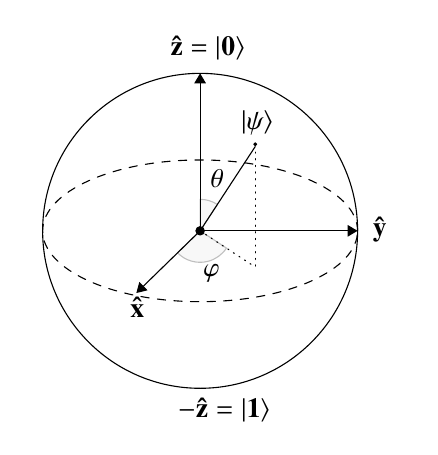
\begin{tikzpicture}[line cap=round, line join=round, >=Triangle]
  \clip(-2.19,-2.49) rectangle (2.66,2.58);
  \draw [shift={(0,0)}, lightgray, fill, fill opacity=0.1] (0,0) -- (56.7:0.4) arc (56.7:90.:0.4) -- cycle;
  \draw [shift={(0,0)}, lightgray, fill, fill opacity=0.1] (0,0) -- (-135.7:0.4) arc (-135.7:-33.2:0.4) -- cycle;
  \draw(0,0) circle (2cm);
  \draw [rotate around={0.:(0.,0.)},dash pattern=on 3pt off 3pt] (0,0) ellipse (2cm and 0.9cm);
  \draw (0,0)-- (0.70,1.07);
  \draw [->] (0,0) -- (0,2);
  \draw [->] (0,0) -- (-0.81,-0.79);
  \draw [->] (0,0) -- (2,0);
  \draw [dotted] (0.7,1)-- (0.7,-0.46);
  \draw [dotted] (0,0)-- (0.7,-0.46);
  \draw (-0.08,-0.3) node[anchor=north west] {$\varphi$};
  \draw (0.01,0.9) node[anchor=north west] {$\theta$};
  \draw (-1.01,-0.72) node[anchor=north west] {$\mathbf {\hat{x}}$};
  \draw (2.07,0.3) node[anchor=north west] {$\mathbf {\hat{y}}$};
  \draw (-0.5,2.6) node[anchor=north west] {$\mathbf {\hat{z}=|0\rangle}$};
  \draw (-0.4,-2) node[anchor=north west] {$-\mathbf {\hat{z}=|1\rangle}$};
  \draw (0.4,1.65) node[anchor=north west] {$|\psi\rangle$};
  \scriptsize
  \draw [fill] (0,0) circle (1.5pt);
  \draw [fill] (0.7,1.1) circle (0.5pt);
\end{tikzpicture}
\caption[Bloch sphere.]{The Bloch sphere is a geometrical representation of the Quantum state in QC.}
\end{figure}


\begin{figure}
\centering
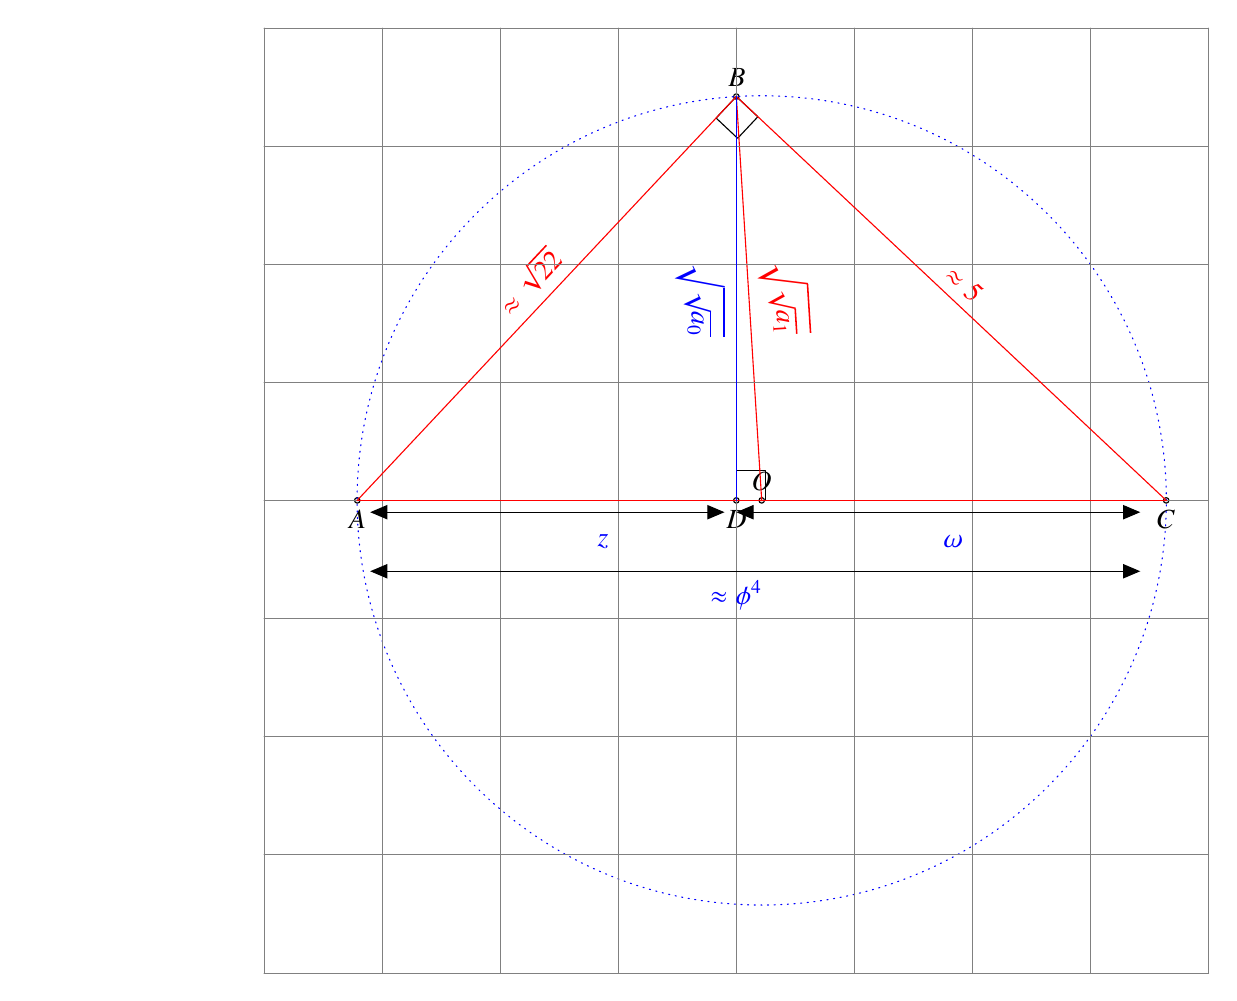
\begin{tikzpicture}[scale=1.5,line cap=round,line join=round,>=triangle 
45,x=1.0cm,y=1.0cm]
%\label{tab:15:table15}
\tkzDefPoint(-3.21,0.0){A} \tkzDefPoint(0.0,3.42){B} \tkzDefPoint(3.64,0.){C} \tkzDefPoint(0.0,0.0){D}
\tkzDrawPoints(A,B,C,D)
\tkzMarkRightAngle(A,B,C)
\tkzMarkRightAngle(B,D,C)
\tkzLabelPoints[below](A,C,D)
\tkzLabelPoints[above](B)
%\tkzMarkAngle[fill=blue!40,size=1.4cm,opacity=.5](C,A,B)
%\tkzLabelAngle[pos=1.6](C,A,B){$\theta$}
\tkzDefMidPoint(A,C) \tkzGetPoint{O}
\coordinate (center) at (O);
\tkzLabelPoints[above](O)
\tkzDrawPoints(O)
\tkzLabelSegment[sloped,above,text=red](A,B){$\approx \sqrt{22}$}
\tkzLabelSegment[sloped,above,text=red](B,C){$\approx 5$}
%\tkzLabelSegment[sloped,below,text=red](A,C){$\approx \phi^{4}$}
\draw[blue, dotted]
      let \p1 =  ($(B)-(center)$),
          \n0 = {veclen(\x1,\y1)}
      in (center) circle(\n0);
\draw[color=red] (B) -- (O);
\tkzDefMidPoint(B,O) \tkzGetPoint{F}
\tkzLabelSegment[sloped,above,text=red](B,O){$\sqrt{\sqrt{a_1}}$}
\draw[color=blue] (B) -- (D);
\tkzDefMidPoint(B,D) \tkzGetPoint{G}
\tkzLabelSegment[sloped,below,text=blue](B,D){$\sqrt{\sqrt{a_0}}$}
\draw[step=1cm,gray,very thin] (-4,-4) grid (4,4);
\draw[color=red] (-3.21,0.) -- (0.,0.);
\draw[color=red] (3.64,0.) -- (0.,0.0);
\draw[color=red] (-3.21,0.) -- (0.,3.42);
\draw[color=red] (0.,3.42) -- (3.64,0.);
\draw[color=blue] (0.,0.) -- (0.,3.42);
%\node [anchor = east] at (0.,1.5) {$\sqrt{\sqrt{a_1}}$};
%\node [anchor = east] at (2.,2.0) {$\approx 5$};
%\node [anchor = east] at (-1.,2.0) {$\approx \sqrt{22}$};
\node [anchor = north,text=blue] at (0.,-0.6) {$\approx \phi^{4}$};
\draw [<->] (-3.1,-0.1) node[left]{} -- (-0.1,-0.1) node[right]{};
\draw [<->] (0.0,-0.1) node[left]{} -- (3.42,-0.1) node[right]{};
\draw [<->] (-3.1,-0.6) node[left]{} -- (3.42,-0.6) node[right]{};
  %\draw [decoration={markings,mark=at position 1 with
   % {\arrow[scale=3,>=stealth reversed]{<}}},postaction={decorate}] (-3.2,-0.3) -- (3.42,-0.3);
\node [anchor = east,text=blue] at (2.,-0.35) {$\omega$};
\node [anchor = east,text=blue] at (-1.,-0.35) {$z$};
\clip(-6.,-0.4) rectangle (0.4,3.4);
%\draw [shift={(-3.2,0.)},color=gray,fill=darkgray,fill opacity=0.1] (0,0) -- (0.:0.6) arc (0.:43.9:0.6) -- cycle;
%\draw[color=gray,fill=darkgray,fill opacity=0.1] (0.,0.42) -- (-0.42,0.42) -- (-0.42,0.) -- (0.,0.) -- cycle; 
%\draw (0.,6.)-- (-4.32,0.);
%\draw (6.,5.52)-- (-4.32,0.);
%\draw (6.,0.)-- (6.,5.52);
%\draw[color=gray] (-3.2,0.4) node {\large $\theta$};
%\draw[color=gray] (0.34,0.33);
%\tkzMarkRightAngle[fill=blue!20](B,F,C)
\end{tikzpicture}
\caption[The Golden Sanchez Triangle.]{Golden Sanchez Triangle.}
\end{figure}

 
 \begin{figure}
\centering
\begin{tikzpicture}[scale=1.25]
%\tkzInit[xmax=6.4, zmax=3.4]
\tkzDefPoint(0.0,0.0){C} \tkzDefPoint(4.9,0.0){B} \tkzDefPoint(3.12,-1.74){A} \tkzDefPoint(1.8,-1.0){q}
\tkzDrawPoints(A,B,C,q)
\tkzDefMidPoint(B,q) \tkzGetPoint{D}
%\tkzDefPoint[label={[text=blue,align=left]right:$z$},xshift=-01mm](2.25,-1.50){F}
%\tkzDefPoint[label={[text=blue,align=left]right:$\omega$},xshift=-01mm](0.75,-0.70){E}
%\tkzDefPoint[label={[text=red,align=left]right:$\sqrt{\omega z}$},xshift=-01mm](2.8,-0.29){D}
%\tkzDefPoint[label={[align=right]right:$4 \cdot \sqrt{(3H\beta/n)}$},xshift=00mm](3.0,-0.79){D}
\tkzLabelSegment[sloped,below,text=red](q,B){$\sqrt{\omega z}$}
\tkzLabelSegment[sloped,below,text=blue](A,q){$z$}
\tkzLabelSegment[sloped,below,text=blue](C,q){$\omega$}
\tkzLabelSegment[sloped,text=blue,xshift=1.5mm,yshift=-07.5mm](A,C){$\phi^4$}
\tkzMarkRightAngle(A,B,C)
\tkzMarkRightAngle(B,q,C)
\tkzLabelPoints[below](A,B,C)
\tkzDrawSegments[red](B,q)
%\tkzLabelPoints[above right](q)
%\tkzMarkAngle[fill=blue!40,size=1.4cm,opacity=.5](C,A,B)
%\tkzLabelAngle[pos=0.6](A,q,B){$\sqrt{\omega z}$}
    %\draw [important line] (0.0,0.) coordinate (A) -- (5.1,-1.3) coordinate (C) node[below, text width=5em] {}
    %\draw [blue] (6.4,0.) coordinate (A) -- (4.,-1.0) coordinate (D) node[below, text width=5em] {$h$}
    %\draw [red] (6.4,0.) coordinate (B) -- (4.,-1.0) coordinate (D) node[below, text width=5em] {$q$}
  \draw (4.9,0,0) coordinate (x) |- (0,1,0) coordinate [midway] (h) coordinate (y) -- (0,1,4.6) coordinate (a) -- (0,0,4.6) coordinate (z) -- (4.9,0,4.6) edge (x) -- (4.9,1,4.6) coordinate (v) edge (h)
  -- (a)  ;
  \draw [dashed] (0,0,0) coordinate (o) edge (x) edge (y) -- (z);
  \draw [dashed] (0,0,0) coordinate (o) edge (x) edge (v) -- (v);
  \draw [blue] (0,0,0)  -- (4.9,0.0,4.6);
  \draw [very thin,black,line join=round] (0,0,0)  -- node [sloped,above,xshift=-0.mm,yshift=-2.mm] {$\approx 4\sqrt 3$} (4.9,1.,4.6);
  %\node [circle, minimum size=2pt, inner sep=0pt, fill, label=135:$4 \cdot \sqrt{(3H\beta/n)}$] at (v) {};
  \node [circle, minimum size=4pt, inner sep=0pt, fill, label=135:o] at (o) {};
  \draw [decoration={markings,mark=at position 1 with
    {\arrow[scale=3,>=stealth]{>}}},postaction={decorate}] (0,0,0) -- (4.9,1,4.6);
  %\draw [<->] (0.2,-0.5) node[left]{} -- (2.2,-1.8) node[below]{$\phi^4$};
  \draw [->] (x) -- +(3pt,0,0) node [midway,above] {$\sqrt{\omega \cdot (\omega+z)}$};
  \draw [->] (y) -- +(0,3pt,0) node [midway,right] {$1$};
  \draw [->] (z) -- +(0,0,3pt) node [midway,above] {$\sqrt{z \cdot (\omega+z)}$};
  %\draw (v) -- ++(0,0,-2) coordinate (d) -- ++(-2,0,0) coordinate (e) -- ++(0,0,2) |- ++(2,-2,0) coordinate [midway] (f) -- ++(0,0,-2) coordinate (g) -- (d);
  %\draw [dashed] (e) -- ++(0,-2,0) coordinate (c) edge (f) -- (g);
  %\node [label=45:C] at (c) {};
  %\draw[red]   (0,0,0) -- (.95,0,0)    node[red,left=6pt]    {$x$};
\end{tikzpicture}
\caption[The Golden Sanchez cuboid properties]{3D perspective of the "Golden-Sanchez" cuboid: Electro-weak / Eddington matrix connection}
\end{figure}


\bibitem{Hirzebruch} Hirzebruch F. Topological methods in algebraic geometry. Springer 1966.\\
\bibitem{Bott} M. Atiyah, R. Bott, V. Patodi, "On the heat equation and the index theorem" Invent. Math. , 19 (1973) pp. 279--330.\\
\bibitem{Singer} M. Atiyah, I. Singer, "The index of elliptic operators IV" Ann. of Math. , 93 (1971) pp. 119--138. \\
\bibitem{Alvarez} L. Alvarez-Gaume, "Supersymmetry and the Atiyah Singer index theorem" Comm. Math. Phys. , 90 (1983) pp. 161--170.\\


\bibitem{Frenkel} I. B. Frenkel, J. Lepowsky, and A. Meurman, “A Natural Representation of the Fischer-Griess Monster With the Modular Function J As Character,” Proc. Natl. Acad. Sci. USA 81 (1984) 3256-3260. 

\bibitem{Witten} Witten E., Three-Dimensional Gravity Revisited arxiv.org/abs/0706.3359 



\bibitem{deVries} Hans de Vries. http://www.chip-architect.com/news/2004/10/04. The Electro-Magnetic coupling constant.html, An exact formula for the Electro Magnetic coupling constant, web page, 2004 Oct 4.\\ 


\bibitem{Atiyah1} Atiyah M. Private Communication (december 2018).\\

\bibitem{Conway} Conway, John Horton; Norton, Simon P. (1979). "Monstrous Moonshine". Bull. London Math. Soc. 11 (3): 308--339.\\
\bibitem{Borcherds} Borcherds, Richard (1992), "Monstrous Moonshine and Monstrous Lie Superalgebras", Invent. Math., 109: 405--444.\\

\bibitem{Shannon} Shannon C.E. « A Mathematical Theory of Communication » Reprinted with corrections from The Bell System Technical Journal, Vol. 27, p. 379–423, 623–656, July, October, 1948.)\\
\bibitem{Stark} Stark H.M. A complete determination of the complex quadratic fields of class-number one, Michigan Math. J., vol. 14,‎ 1967, p. 1-27  \\
\bibitem{Lovelace} Lovelace C. (1971) Pomeron form factors and dual Regee cuts, Physics Letters B34 (6) 500-506.\\
\bibitem{Apostol} Apostol T. Modular functions and Dirichlet Series in Number Theory. Springler-Verlag. New-York (1990).\\

\bibitem{Shlay} Shray J. (1994) Octonions and Supersymmetry, PhD thesis.  http://ir.library.oregonstate.edu/xmlui/handle/1957/35649. \\
 
\bibitem{Hooft} Hooft 't Th Holographic Principle. ArXiv: hep-th/003004 (2000). \\
\bibitem{Bousso} Bousso R., The Holographic Principle, Review of Modern Physics, vol 74, p.834 (2002).\\
 
\bibitem{Durham} Durham I.T. 2006, Sir Arthur Eddington and the Foundations of Modern Physics arXiv:quant-ph/0603146v1  p.117.
\bibitem{Sanchez2} Sanchez F.M., Kotov V. and Bizouard C., 'Towards a synthesis of two cosmologies: the steady- state flickering Universe'. Journal of Cosmology, vol 17. (2011).\\


\bibitem{Carr} Carr B.J. and Rees M. J. , “The anthropic principle and the structure of the physical world”, Nature 278, 605-612 (1979).\\
\bibitem{Sanchez3} F.M. Sanchez. Coherent Cosmology Vixra.org,1601.0011. Springer International Publishing AG 2017. A. Tadjer et al. (eds.), Quantum Systems in Physics, Chemistry, and Biology, Progress in Theoretical Chemistry and Physics 30, pp. 375--407. \\ 
\bibitem{LaGuer} Gueroult.L, 49 methods for computing the Hubble Radius with Jupyter https://mybinder.org/v2/gh/LaGuer/hubble-radius/master \\

\bibitem{Lenz} Friedrich Lenz, The Ratio of Proton and Electron Masses, Phys. Rev. 82, 554 - 1951.\\

%\bibitem{Lecompte} Sanchez, F and Lecompte, C, ``Q-Switched $Nd^{3+}$ Glass Laser of Variable Temporal Coherence, Applied optics'', vol.13, p1071-6, 05.1974, DOI: 10.1364/AO.13.001071 \\


%\bibitem{Mainfray} Lecompte, C. and Mainfray, G. and Manus, C. and Sanchez, F., ``Laser temporal-coherence effects on multiphoton ionization processes'', Phys. Rev. A, vol.11, 03.1975, DOI: 10.1103/PhysRevA.11.1009 \\

%\bibitem{Manus} Mainfray, G. and Manus, C. and Sanchez, F., ``Experimental Demonstration of Laser Temporal Coherence Effects on Multiphoton Ionization Processes'', Quantum Electronics, IEEE Journal of, vol.QE10, p707, 10.1974, DOI:0.1109/JQE.1974.1068290 \\


%\bibitem{SanchezF} Sanchez, F., ``High-order multimode radiation statistics of aTEM00Q-switched neodymium laser'', Il Nuovo Cimento B, vol.27, p305--322, 06.1975, DOI:10.1007/BF02738949 \\



\bibitem{Nist} ``2018 CODATA Value: Newtonian constant of gravitation''. The NIST Reference on Constants, Units, and Uncertainty. NIST. 20 May 2019. Retrieved 20 May 2019. https://www.physics.nist.gov/cgi-bin/cuu/Value?bg \\

%\bibitem{Haramein} Haramein N. ``The Schwarzschild Proton'', 2011, p95--100, vol.60, DOI: 10.1063/1.3527190. \\

\bibitem{Haramein} Haramein N., Val Baker A. ``Resolving the Vacuum catastrophe. A Generalised Holographic Approach. Journal of High Energy Physics, Gravitation and Cosmology'', 2019, 5, 412-424 \\ 

\bibitem{Val} Val Baker A. ``The puzzle of the proton'', DOI : 1031219/osf.io/myfxh \\

\bibitem{Maruani} Jean Maruani. ``The Dirac Electron: From Quantum Chemistry to Holistic Cosmology'' in Journal of the Chinese Chemical Society, vol.63 issue 1, Taipei, Wiley VCH Verlag GmbH, 2016, 33--48 p. DOI: https://doi.org/10.1002/jccs.201500374 \\

\bibitem{oeis1} OEIS Foundation Inc. The on-line encyclopedia of integer sequences,https://oeis.org/A180873, Sep 22 2010.

\bibitem{Veysseyre} Veysseyre R., Veysseyre H., and Weigel D. "Nombre de types d’opérations ponctuelles de symétrie cristallographiques dans l’espace E^{n} . (Number of types of crystallographic point symmetry operations of space E^{n} )", Comptes Rendus de l’Académie des Sciences. Série II (Jan.1990).\\

\bibitem{Weigel} Veysseyre R., Veysseyre H., and Weigel D. "Counting, types and symbols of crystallographic Point Symmetry
Operations of space E n" AAECC 5, 53–70 (1992) DOI: 10.1007/BF01196625 ISBN: 0938-1279.\\







